The results section of this paper is split up in two parts. Firstly, HRA per player is computed, analyzed and aggregated considering various factors, including time, team and manager. Secondly, the drivers of home advantage at an individual player level are investigated using linear regression and random forest regression.

\subsection{Home Rating Advantage}

\subsubsection{Home Advantage over the Seasons}
Table \ref{tab:hra_full_sample} shows home advantage over the full sample. As a quick reminder, the concept of home advantage in this study is based on the utilization of home rating advantage (HRA). A distinction is made between the unweighted and weighted average HRA. The unweighted HRA average does not take into account the number of match-pairs an observation for HRA is based on. The weighted HRA does take into account the number of match-pairs an observation is based on. As illustrated in Table \ref{tab:hra_full_sample}, the two averages are very similar. HRA over the whole sample is around 0.14 points. This is a modest result, given that player ratings are given on a continuous scale of 1--10. However, this result is still a clear indication that home advantage exists on an individual player basis. \\ 

\begin{table}[htbp]
    \begin{spacing}{1.5}
    \centering
    \small
    \caption{Player-based home advantage in the English Premier League, 2009--2023}
    \label{tab:hra_full_sample}%
    \begin{tabular}{p{5cm}p{2cm}}
        \toprule
        \toprule
        \textbf{Average type} & \multicolumn{1}{l}{\textbf{HRA}} \\
        \midrule
        Unweighted Average & 0.143751 \\
        Weighted Average & 0.143750 \\
        \bottomrule
        \bottomrule
    \end{tabular}%
    \end{spacing}
\end{table}%

\noindent
Figure \ref{fig:hra_over_the_seasons} shows the development of home advantage in the English Premier League over the seasons. Home advantage was highest in the 2009/2010 season and lowest in the 2020/2021 season. The latter result is interesting, as this was the season which was played under strict COVID-19 crowd restrictions. Only a small number of spectators were allowed into the stadiums during this season. This is a first indication that the presence of fans has a large impact on the home advantage experienced by players. Furthermore, we see that there seems to be a downward trend in home advantage over the years right up to the 2020/2021 season. This result is in line with \shortciteA{peeters_2021}, who also showed that there has been a secular decline in home advantage in English professional football over the years.

\begin{figure}[htbp]
    \centering
    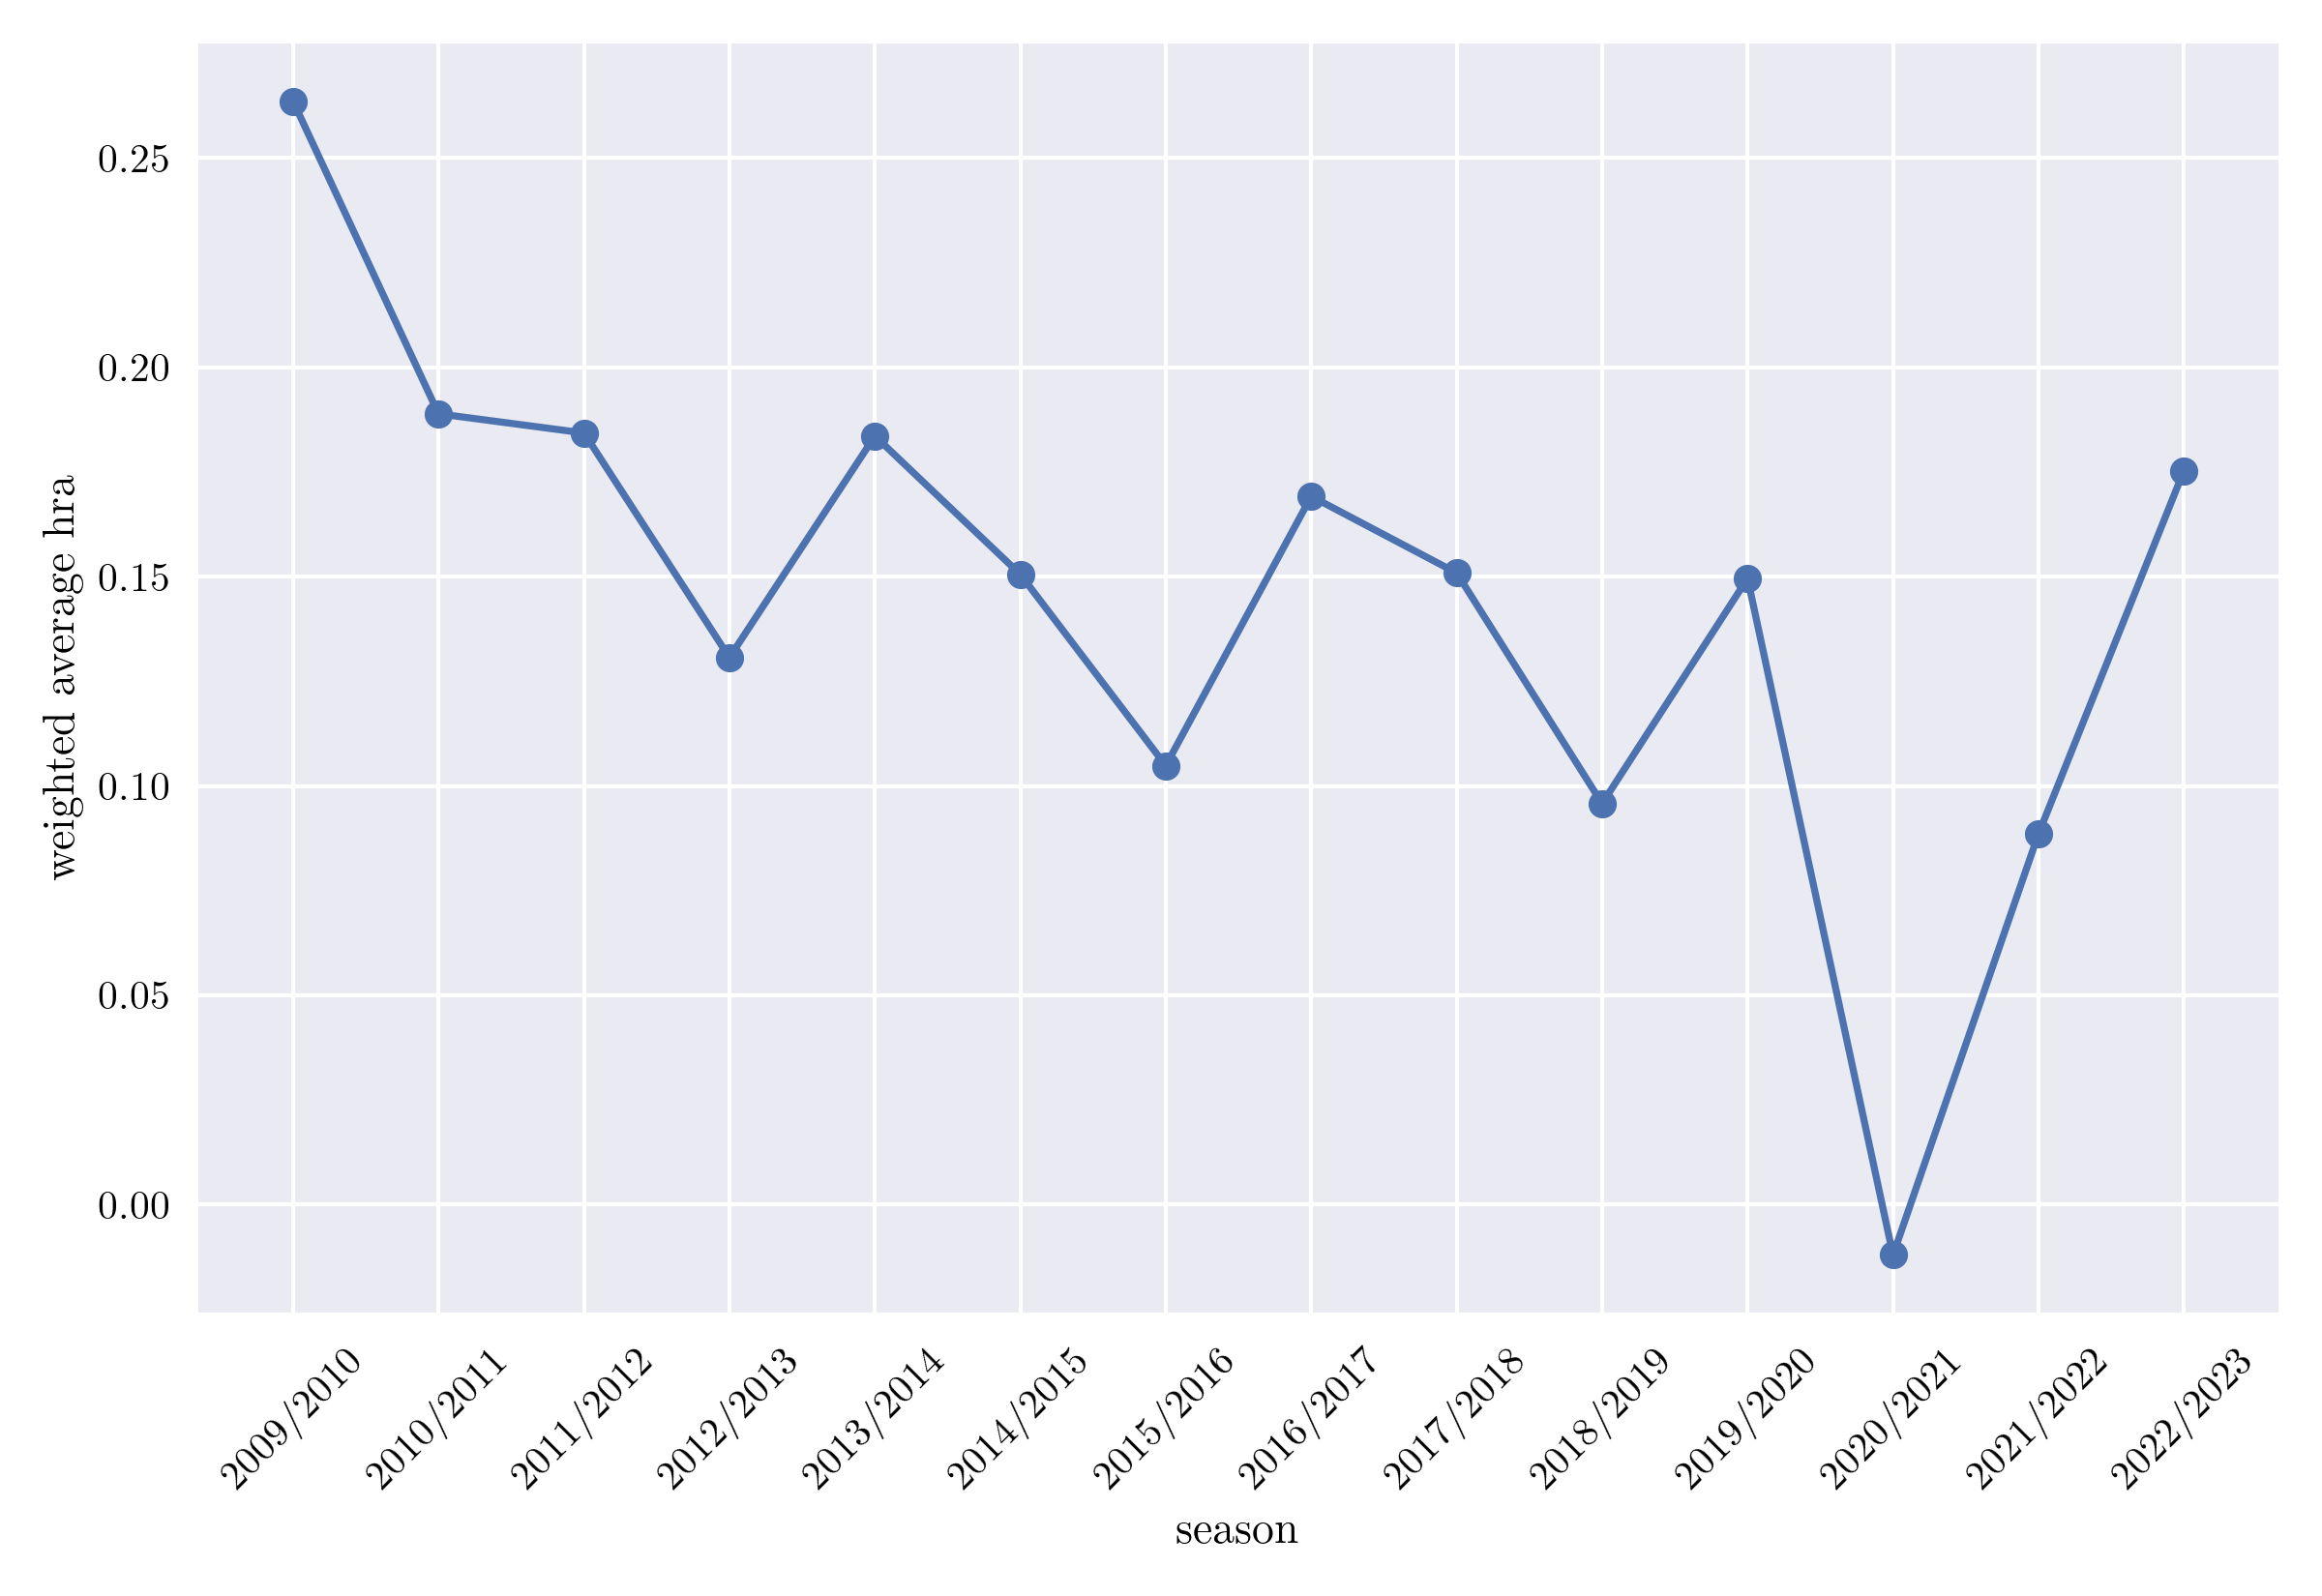
\includegraphics[width=0.8\textwidth]{attachments/average_hra_per_season.png}
    \caption{Home advantage in the English Premier League over the years, 2009--2023}
    \label{fig:hra_over_the_seasons}
\end{figure}

\subsubsection{HRA per Team}
In terms of fairness of the competition, total average home advantage over the seasons is not very useful. The round robin format of the EPL ensures that the total effect of home advantage is cancelled out across clubs. Instead, home advantage per team is analyzed. Table \ref{tab:hra_per_team} gives an overview of the aggregated HRA per team in the EPL over the period 2009--2023. Note that this Table only includes teams that played at least seven seasons in the EPL over the given time period. There are stark differences in the HRA enjoyed by players on different teams. Liverpool has the highest weighted average HRA with a value of 0.212 and Crystal Palace the lowest with a value of 0.033. So, the home advantage that is on average enjoyed by Liverpool players is more than six times as high as that of Crystal Palace players in terms of home rating advantage.

\begin{table}[htbp]
    \begin{spacing}{1.5}
    \small
    \centering
    \caption{Home advantage per team in the EPL, 2009--2023}
    \label{tab:hra_per_team}%
    \begin{tabular}{lrrrr}
        \toprule
        \toprule
        \textbf{Team}  & \multicolumn{1}{l}{\textbf{Season count}} &       & \multicolumn{2}{c}{\textbf{Average HRA}} \\
        \cmidrule{4-5}          &       &       & \multicolumn{1}{l}{\textbf{Unweighted}} & \multicolumn{1}{l}{\textbf{Weighted}} \\
        \midrule
        Arsenal & 14    &       & 0.202 & 0.194 \\
        Aston Villa & 11    &       & 0.051 & 0.045 \\
        Burnley & 8     &       & 0.067 & 0.068 \\
        Chelsea & 14    &       & 0.189 & 0.189 \\
        Crystal Palace & 10    &       & 0.036 & 0.033 \\
        Everton & 14    &       & 0.174 & 0.171 \\
        Fulham & 8     &       & 0.093 & 0.104 \\
        Leicester City & 9     &       & 0.130 & 0.124 \\
        Liverpool & 14    &       & 0.214 & 0.212 \\
        Manchester City & 14    &       & 0.189 & 0.187 \\
        Manchester United & 14    &       & 0.173 & 0.175 \\
        Newcastle United & 12    &       & 0.163 & 0.167 \\
        Southampton & 11    &       & 0.087 & 0.090 \\
        Stoke City & 9     &       & 0.139 & 0.137 \\
        Sunderland & 8     &       & 0.148 & 0.159 \\
        Swansea City & 7     &       & 0.194 & 0.180 \\
        Tottenham Hotspur & 14    &       & 0.210 & 0.200 \\
        West Bromwich Albion & 9     &       & 0.087 & 0.085 \\
        West Ham United & 13    &       & 0.134 & 0.133 \\
        Wolverhampton Wanderers & 8     &       & 0.103 & 0.095 \\
        \bottomrule
        \bottomrule
        \multicolumn{5}{p{12cm}}{\footnotesize\textit{Note.} Teams are only included if they have competed in at least 7 out of the 14 seasons under consideration.}
    \end{tabular}
    \end{spacing}
\end{table}%

\subsubsection{Players and HRA}
In addition to examining heterogeneity among teams, heterogeneity in home advantage among players is also investigated. This analysis is possible due to the fact that the HRA metrics are all player based. Table \ref{tab:hra_per_player} shows HRA per player for all players that have played at least three seasons and thirty home-away game pairs. When comparing panel a. and panel b. in Table \ref{tab:hra_per_player} big differences in HRA per player are observed. Furthermore, when looking at panel c. there is no clear indication that experienced players enjoy more or less HRA compared to the (unweighted) average HRA over the whole sample of 0.14. In Section \ref{subsec:driver_of_home_advantage} the underlying factors relating to heterogeneity in HRA among players will be investigated.

\begin{table}[htbp]
    \begin{spacing}{1.5}
    \small
    \centering
    \caption{Home advantage per player in the EPL, 2009--2023}
    \label{tab:hra_per_player}
    \begin{tabular}{lrrrrr}
        \toprule
        \toprule
        \textbf{Player} & \multicolumn{2}{c}{\textbf{Experience}} &       & \multicolumn{2}{c}{\textbf{Average HRA}} \\
        \cmidrule{2-3}\cmidrule{5-6}          & \multicolumn{1}{l}{\textbf{Season count}} & \multicolumn{1}{l}{\textbf{Game pairs}} &       & \multicolumn{1}{l}{\textbf{Unweighted}} & \multicolumn{1}{l}{\textbf{Weighted}} \\
        \midrule
        \multicolumn{6}{c}{a. Top 10} \\
        \midrule
        Leroy Fer & 4     & 31    &       & 0.857 & 0.717 \\
        Benoit Assou-Ekotto & 4     & 38    &       & 0.631 & 0.640 \\
        Mesut Ozil & 7     & 57    &       & 0.654 & 0.593 \\
        Samir Nasri & 6     & 49    &       & 0.559 & 0.575 \\
        Kevin De Bruyne & 7     & 69    &       & 0.554 & 0.561 \\
        Joey Barton & 3     & 35    &       & 0.540 & 0.547 \\
        Olivier Giroud & 5     & 40    &       & 0.333 & 0.503 \\
        Dirk Kuyt & 3     & 36    &       & 0.374 & 0.501 \\
        Clint Dempsey & 4     & 47    &       & 0.355 & 0.466 \\
        Sadio Mane & 8     & 93    &       & 0.530 & 0.464 \\
        \midrule
        \multicolumn{6}{c}{b. Bottom 10} \\
        \midrule
        Shane Duffy & 4     & 37    &       & -0.818 & -0.549 \\
        Emiliano Martinez & 3     & 53    &       & -0.342 & -0.340 \\
        Mame Diouf & 4     & 31    &       & -0.295 & -0.263 \\
        Yves Bissouma & 5     & 34    &       & -0.305 & -0.249 \\
        Adrian & 5     & 38    &       & -0.750 & -0.246 \\
        Artur Boruc & 4     & 44    &       & -0.118 & -0.238 \\
        Nick Pope & 5     & 82    &       & -0.263 & -0.237 \\
        Tom Cleverley & 8     & 40    &       & -0.308 & -0.234 \\
        Gabriel Magalhaes & 3     & 39    &       & -0.303 & -0.213 \\
        Mathew Ryan & 3     & 52    &       & -0.197 & -0.201 \\
        \midrule
        \multicolumn{6}{c}{c. Most experienced} \\
        \midrule
        Jordan Henderson & 14    & 123   &       & 0.216 & 0.281 \\
        Jonny Evans & 13    & 95    &       & -0.029 & -0.026 \\
        James Milner & 13    & 82    &       & 0.370 & 0.247 \\
        David de Gea & 12    & 188   &       & -0.084 & -0.049 \\
        Kyle Walker & 12    & 131   &       & 0.081 & 0.073 \\
        Seamus Coleman & 12    & 107   &       & 0.231 & 0.230 \\
        Hugo Lloris & 11    & 156   &       & 0.117 & 0.102 \\
        Cesar Azpilicueta & 11    & 136   &       & 0.121 & 0.135 \\
        Mark Noble & 11    & 117   &       & 0.239 & 0.278 \\
        Gary Cahill & 11    & 103   &       & -0.041 & 0.054 \\
        \bottomrule
        \bottomrule
        \multicolumn{6}{p{14cm}}{\footnotesize\textit{Note.} Players are only included if they have competed in at least three seasons and played at least thirty home-away game pairs.}
    \end{tabular}
    \end{spacing}
\end{table}


\subsubsection{Managers and HRA}
In a similar fashion to the previous subsection, HRA is analyzed but now per manager. Table \ref{tab:hra_per_manager} shows HRA per manager for all managers that have at least three seasons of experience in the EPL. From panel c. it becomes clear that there is no direct relation between the experience of a manager and the home advantage the manager experiences with his players. The weighted average HRA over the whole sample equals 0.14. For some managers in panel c. HRA is higher than 0.14 and for other managers HRA is lower than 0.14.

% Table generated by Excel2LaTeX from sheet 'Results'
\begin{table}[htbp]
    \begin{spacing}{1.5}
    \small
    \centering
    \caption{Home advantage per manager in the EPL, 2009--2023}
    \label{tab:hra_per_manager}
    \begin{tabular}{lrrrr}
        \toprule
        \toprule
        \textbf{Manager} & \multicolumn{1}{l}{\textbf{Season count}} &       & \multicolumn{2}{c}{\textbf{Average HRA}} \\
        \cmidrule{4-5}          &       &       & \multicolumn{1}{l}{\textbf{Unweighted}} & \multicolumn{1}{l}{\textbf{Weighted}} \\
        \midrule
        \multicolumn{5}{c}{a. Top 10} \\
        \midrule
        Ronald Koeman & 3     &       & 0.237 & 0.283 \\
        Carlo Ancelotti & 4     &       & 0.416 & 0.257 \\
        Arsene Wenger & 9     &       & 0.234 & 0.256 \\
        Alex McLeish & 3     &       & 0.212 & 0.236 \\
        Manuel Pellegrini & 4     &       & 0.267 & 0.232 \\
        Steve Bruce & 6     &       & 0.161 & 0.209 \\
        Roberto Mancini & 4     &       & 0.257 & 0.208 \\
        Harry Redknapp & 4     &       & 0.074 & 0.204 \\
        Brendan Rodgers & 8     &       & 0.178 & 0.186 \\
        Rafael Benitez & 5     &       & 0.180 & 0.183 \\
        \midrule
        \multicolumn{5}{c}{b. Bottom 10} \\
        \midrule
        Dean Smith & 4     &       & 0.021 & 0.005 \\
        Graham Potter & 4     &       & 0.075 & 0.018 \\
        Paul Lambert & 4     &       & 0.010 & 0.018 \\
        Marco Silva & 3     &       & 0.008 & 0.028 \\
        Sean Dyche & 8     &       & 0.029 & 0.045 \\
        Ole Gunnar Solskjaer & 4     &       & 0.102 & 0.091 \\
        Roy Hodgson & 9     &       & 0.103 & 0.093 \\
        Nuno Espirito Santo & 3     &       & 0.119 & 0.094 \\
        Eddie Howe & 7     &       & 0.141 & 0.095 \\
        David Moyes & 11    &       & 0.063 & 0.102 \\
        \midrule
        \multicolumn{5}{c}{c. Most experienced} \\
        \midrule
        David Moyes & 11    &       & 0.063 & 0.102 \\
        Arsene Wenger & 9     &       & 0.234 & 0.256 \\
        Sam Allardyce & 9     &       & 0.158 & 0.171 \\
        Roy Hodgson & 9     &       & 0.103 & 0.093 \\
        Tony Pulis & 8     &       & 0.142 & 0.151 \\
        Jurgen Klopp & 8     &       & 0.152 & 0.177 \\
        Sean Dyche & 8     &       & 0.029 & 0.045 \\
        Brendan Rodgers & 8     &       & 0.178 & 0.186 \\
        Roberto Martinez & 7     &       & 0.164 & 0.136 \\
        Pep Guardiola & 7     &       & 0.125 & 0.152 \\
        \bottomrule
        \bottomrule
        \multicolumn{5}{p{12cm}}{\footnotesize\textit{Note.} Managers are only included if they have coached a team in at least three seasons.}
    \end{tabular}
    \end{spacing}
\end{table}

\subsection{Drivers of Home Advantage at the Player Level}
\label{subsec:driver_of_home_advantage}
In this section the drivers of home advantage at an individual player level are investigated. This analysis is based on the model presented in Equation \ref{eq:general_hra_model}. The model is estimated using two different methods: linear regression and random forest regression. Further elaboration and detailed information can be found in Section \ref{subsec:drivers_of_home_advantage_methodology}. Additionally, some sensitivity analysis is performed. The model-estimation methods are applied to two different datasets. Firstly, the methods are applied to the full dataset. Secondly, the methods are applied to a filtered dataset. Here the filtered dataset only contains observations where the number of home-away match pairs per player is at least 10. This dataset may give more accurate results, since now only players that have played at least half of the season are included in the analysis. This could potentially mitigate issues like the form of the player or injuries, since players with only one or two home-away match pairs have these matches spread out across the year.

\subsubsection{Linear Regression}
Table \ref{tab:lr_parameters} shows the parameter estimates for Equation \ref{eq:lr_hra_model} estimated using the weighted least squares (WLS) criterion. \\

\begin{table}[htbp]
    \begin{spacing}{1.5}
    \small
    \centering
    \caption{Linear regression results for the relationship between seasonal home advantage per player and several player characteristics in the English Premier League, 2009--2023}
    \label{tab:lr_parameters}
    \begin{tabular}{p{7cm}rr}
        \toprule
        \toprule
        \textbf{Variable} & \multicolumn{2}{c}{\textbf{Sample}} \\
        \cmidrule{2-3}          & \multicolumn{1}{c}{\textbf{Full}} & \multicolumn{1}{c}{\textbf{Filtered}} \\
        \midrule
        Promoted & 0.0194 & $0.0332^{*}$ \\
              & (0.0170) & (0.0213) \\
        Captain & 0.0165 & 0.0151 \\
              & (0.0194) & (0.0228) \\
        Goalkeeper & $-0.1550^{****}$ & $-0.1695^{****}$ \\
              & (0.0316) & (0.0403) \\
        Defender & $-0.0638^{****}$ & $-0.0895^{****}$ \\
              & (0.0196) & (0.0269) \\
        Midfielder & -0.0022 & -0.0197 \\
              & (0.0181) & (0.0250) \\
        British & $0.0167^{*}$ & 0.0041 \\
              & (0.0113) & (0.0146) \\
        Average home attendance (x10,000) & $0.0302^{****}$ & $0.0316^{****}$ \\
              & (0.0045) & (0.0057) \\
        Quality & 0.0013 & 0.0024 \\
              & (0.0016) & (0.0021) \\
        Skill moves & $0.0213^{***}$ & $0.0186^{*}$ \\
              & (0.0092) & (0.0118) \\
        Age   & 0.0006 & -0.0008 \\
              & (0.0015) & (0.0020) \\
        Trend & $-0.0085^{****}$ & $-0.0086^{****}$ \\
              & (0.0016) & (0.0020) \\
        Observations & 4438  & 1619 \\
        $R^2$    & 0.084 & 0.164 \\
        \bottomrule
        \bottomrule
        \multicolumn{3}{p{12cm}}{\footnotesize\textit{Note.} Standard errors are in parentheses; HC1 robust standard errors are used; parameters for team-fixed effects and constants are not included; * p\textless 0.15, ** p\textless 0.10, *** p\textless0.05, **** p\textless0.01.}
    \end{tabular}
    \end{spacing}
\end{table}%

\noindent
When considering the filtered sample parameter estimates by looking at Table \ref{tab:lr_parameters} we see that being promoted has a small positive effect on home advantage for a player, however it is only significant at a 15\% level. Being the captain on a team does not seem to have any contribution to the home advantage enjoyed by a player. Furthermore, it is interesting to see that goalkeepers and defenders enjoy significantly less home advantage than midfielders and attackers. There is no indication that British players experience more home advantage than foreign players. Average home attendance has a highly significant positive effect on the home advantage enjoyed by a player. There is no indication that higher quality players experience more home advantage than lower quality players. Additionally, it appears that skill moves and flair are positively related to a player's home advantage. However, this result is only significant at a 15\% level. The age of a player does not seem to have any effect on the home advantage of a player. Finally, there is strong evidence that home advantage on an individual player basis has decreased over the period 2009--2023. The trend variable is highly significant and has a negative coefficient. \\

\noindent
Table \ref{tab:lr_parameters} also contains the full sample parameter estimates. Two differences are observed compared to the filtered sample parameter estimates. Firstly, the promoted variable is no longer significant. Secondly, the British boolean variable is now significant at a 15\% level, and carries a positive effect to home advantage. The variables for the playing position in the field, the average home attendance, skill moves and the trend remain highly significant over both samples. \\

\noindent
Finally, as a robustness check, the model in Equation \ref{eq:lr_hra_model} is also fitted using season-fixed effects instead of the trend variable, to analyze the stability of the parameter coefficients and their significance. The parameter estimates obtained from the model with season-fixed effects are not significantly different from those presented in Table \ref{tab:lr_parameters}. However, one notable change is that the promotion variable is no longer statistically significant for the filtered sample at a 15\% level.
\newpage

\subsubsection{Random Forest Regression}
Table \ref{tab:forecasting_metrics} shows a comparison of the in-sample fit of between the LR-based model and the RFR-based model. Three metrics are used for this purpose: \textit{mean squared error} (MSE), \textit{mean absolute error} (MAE) and $R^2$. The results are interesting for two reasons. Firstly, the results clearly show that the explanatory power of the model becomes larger when switching to the filtered sample. This is shown by the higher $R^2$ values and lower MSE and MAE values. Secondly, Table \ref{tab:forecasting_metrics} shows that the RFR-based model beats the LR-based model in terms of in-sample fit for every performance metric for both datasets. This shows that the explanatory power of the RFR-based model is higher than that of the more traditional LR-based model.

\begin{table}[htbp]
    \begin{spacing}{1.5}
    \small
    \centering
    \caption{In-sample fit comparison, linear regression vs random forest regression}
    \label{tab:forecasting_metrics}
    \begin{tabular}{p{2cm}rrrrr}
        \toprule
        \toprule
        \textbf{Metric} & \multicolumn{2}{c}{\textbf{LR}} &       & \multicolumn{2}{c}{\textbf{RFR}} \\
        \cmidrule{2-3}\cmidrule{5-6}          & \multicolumn{1}{l}{\textbf{Full sample}} & \multicolumn{1}{l}{\textbf{Filtered sample}} &       & \multicolumn{1}{l}{\textbf{Full sample}} & \multicolumn{1}{l}{\textbf{Filtered sample}} \\
        \midrule
        MSE   & 0.111 & 0.062 &       & 0.105 & 0.056 \\
        MAE   & 0.242 & 0.193 &       & 0.236 & 0.187 \\
        $R^2$    & 0.084 & 0.164 &       & 0.132 & 0.236 \\
        \bottomrule
        \bottomrule
    \end{tabular}
\end{spacing}
\end{table}

\noindent
Table \ref{tab:var_importance_full_sample} and Table \ref{tab:var_importance_filtered_sample} show the variable importance (VI) of the ten most important explanatory variables for the RFR-based model for the full and filtered dataset respectively. For both datasets the average home attendance variable is the most important, accounting for about 18\% of the total explanation power of the model. Furthermore, the set of top ten variables is the same in both Tables, however the order is a bit different. The five most important variables have a total explanation power of about 60\% relative to the total model explanation power. While the order of the variables is slightly different between Table \ref{tab:var_importance_full_sample} and Table \ref{tab:var_importance_filtered_sample}, the actual magnitudes of the variable importance per variable are not that different between the Tables. Notably, in the RFR-based model, player quality and age emerge as significant factors, both ranking within the top five most important explanatory variables in terms of variable importance. This is in contrast to the LR-based model results in Table \ref{tab:lr_parameters}, here player quality and age are both not statistically significant on any level. \\

\begin{table}[htbp]
    \begin{spacing}{1.5}
    \small
    \centering
    \caption{Variable importance of the random forest regression based model (full sample)}
    \label{tab:var_importance_full_sample}
    \begin{tabular}{lrr}
        \toprule
        \toprule
        \textbf{Variable} & \multicolumn{1}{l}{\textbf{Variable importance}} & \multicolumn{1}{l}{\textbf{Cumulative importance}} \\
        \midrule
        Average home attendance & 0.178 & 0.178 \\
        Skill moves & 0.112 & 0.290 \\
        Trend & 0.111 & 0.402 \\
        Quality & 0.109 & 0.511 \\
        Age   & 0.077 & 0.588 \\
        Goalkeeper & 0.077 & 0.665 \\
        Midfielder & 0.035 & 0.699 \\
        Defender & 0.033 & 0.732 \\
        Attacker & 0.025 & 0.757 \\
        British & 0.021 & 0.779 \\
        \bottomrule
        \bottomrule
        \multicolumn{3}{p{13cm}}{\footnotesize\textit{Note.} Variable importance per explanatory variable is calculated as the total reduction in the sum of squared errors brought by that variable (Gini importance).}
    \end{tabular}
    \end{spacing}
\end{table}

\begin{table}[htbp]
    \begin{spacing}{1.5}
    \small
    \centering
    \caption{Variable importance of the random forest regression based model (filtered sample)}
    \label{tab:var_importance_filtered_sample}
    \begin{tabular}{lrr}
        \toprule
        \toprule
        \textbf{Variable} & \multicolumn{1}{l}{\textbf{Variable importance}} & \multicolumn{1}{l}{\textbf{Cumulative importance}} \\
        \midrule
        Average home attendance & 0.171 & 0.171 \\
        Quality & 0.110 & 0.281 \\
        Trend & 0.106 & 0.387 \\
        Skill moves & 0.096 & 0.483 \\
        Age   & 0.085 & 0.568 \\
        Goalkeeper & 0.064 & 0.632 \\
        Attacker & 0.033 & 0.665 \\
        Midfielder & 0.032 & 0.697 \\
        Defender & 0.028 & 0.725 \\
        British & 0.019 & 0.744 \\
        \bottomrule
        \bottomrule
        \multicolumn{3}{p{13cm}}{\footnotesize\textit{Note.} Variable importance per explanatory variable is calculated as the total reduction in the sum of squared errors brought by that variable (Gini importance).}
    \end{tabular}
    \end{spacing}
\end{table}

\noindent
Now that the variable importance of the explanatory variables in the RFR-based model have been investigated, the actual effect of the explanatory variables on home advantage is analyzed. Figure \ref{fig:pd_plots_1} and Figure \ref{fig:pd_plots_2} show the partial dependence plots for the most important variables in terms of variable importance. Additionally, the effect of the playing position of a player is examined. Both the full dataset and the filtered dataset are considered. Just like in the LR-based model, average home attendance is positively related to home advantage. The difference between a near empty stadium and a stadium packed with nearly 70,000 fans is roughly 0.08 HRA points. Furthermore, the relationship between average home attendance and home advantage exhibits a monotonically increasing pattern with a decreasing marginal effect. Moreover, higher player quality is related to higher home advantage for a player. This is especially true for the top twenty percent players, here we see a steep increase in HRA from about 0.13 to 0.21. It seems that the rare players of exceptional quality enjoy a lot more home advantage than average quality players. The relation between the home advantage a player enjoys and his quality is also strongly non-linear, which may be one of the reasons the LR-based model did not find it to be statistically significant. The trend variable is negatively related to home advantage per player. This result is similar to the LR-based model. Furthermore, more skilled players enjoy more home advantage according to the RFR-based model. This result was also found in the LR-based model. Figure \ref{fig:pd_plots_2} also shows that as players get older, the home advantage they enjoy decreases. This relation is not monotonically decreasing for the whole sample however. The negative effect of player age on home advantage was also not found in the LR-based model. Finally, the partial dependence plot of the playing position reveals that attackers and midfielders enjoy more home advantage than defenders and goalkeepers. This result was also found in the LR-based model.

\begin{figure}
    \centering
    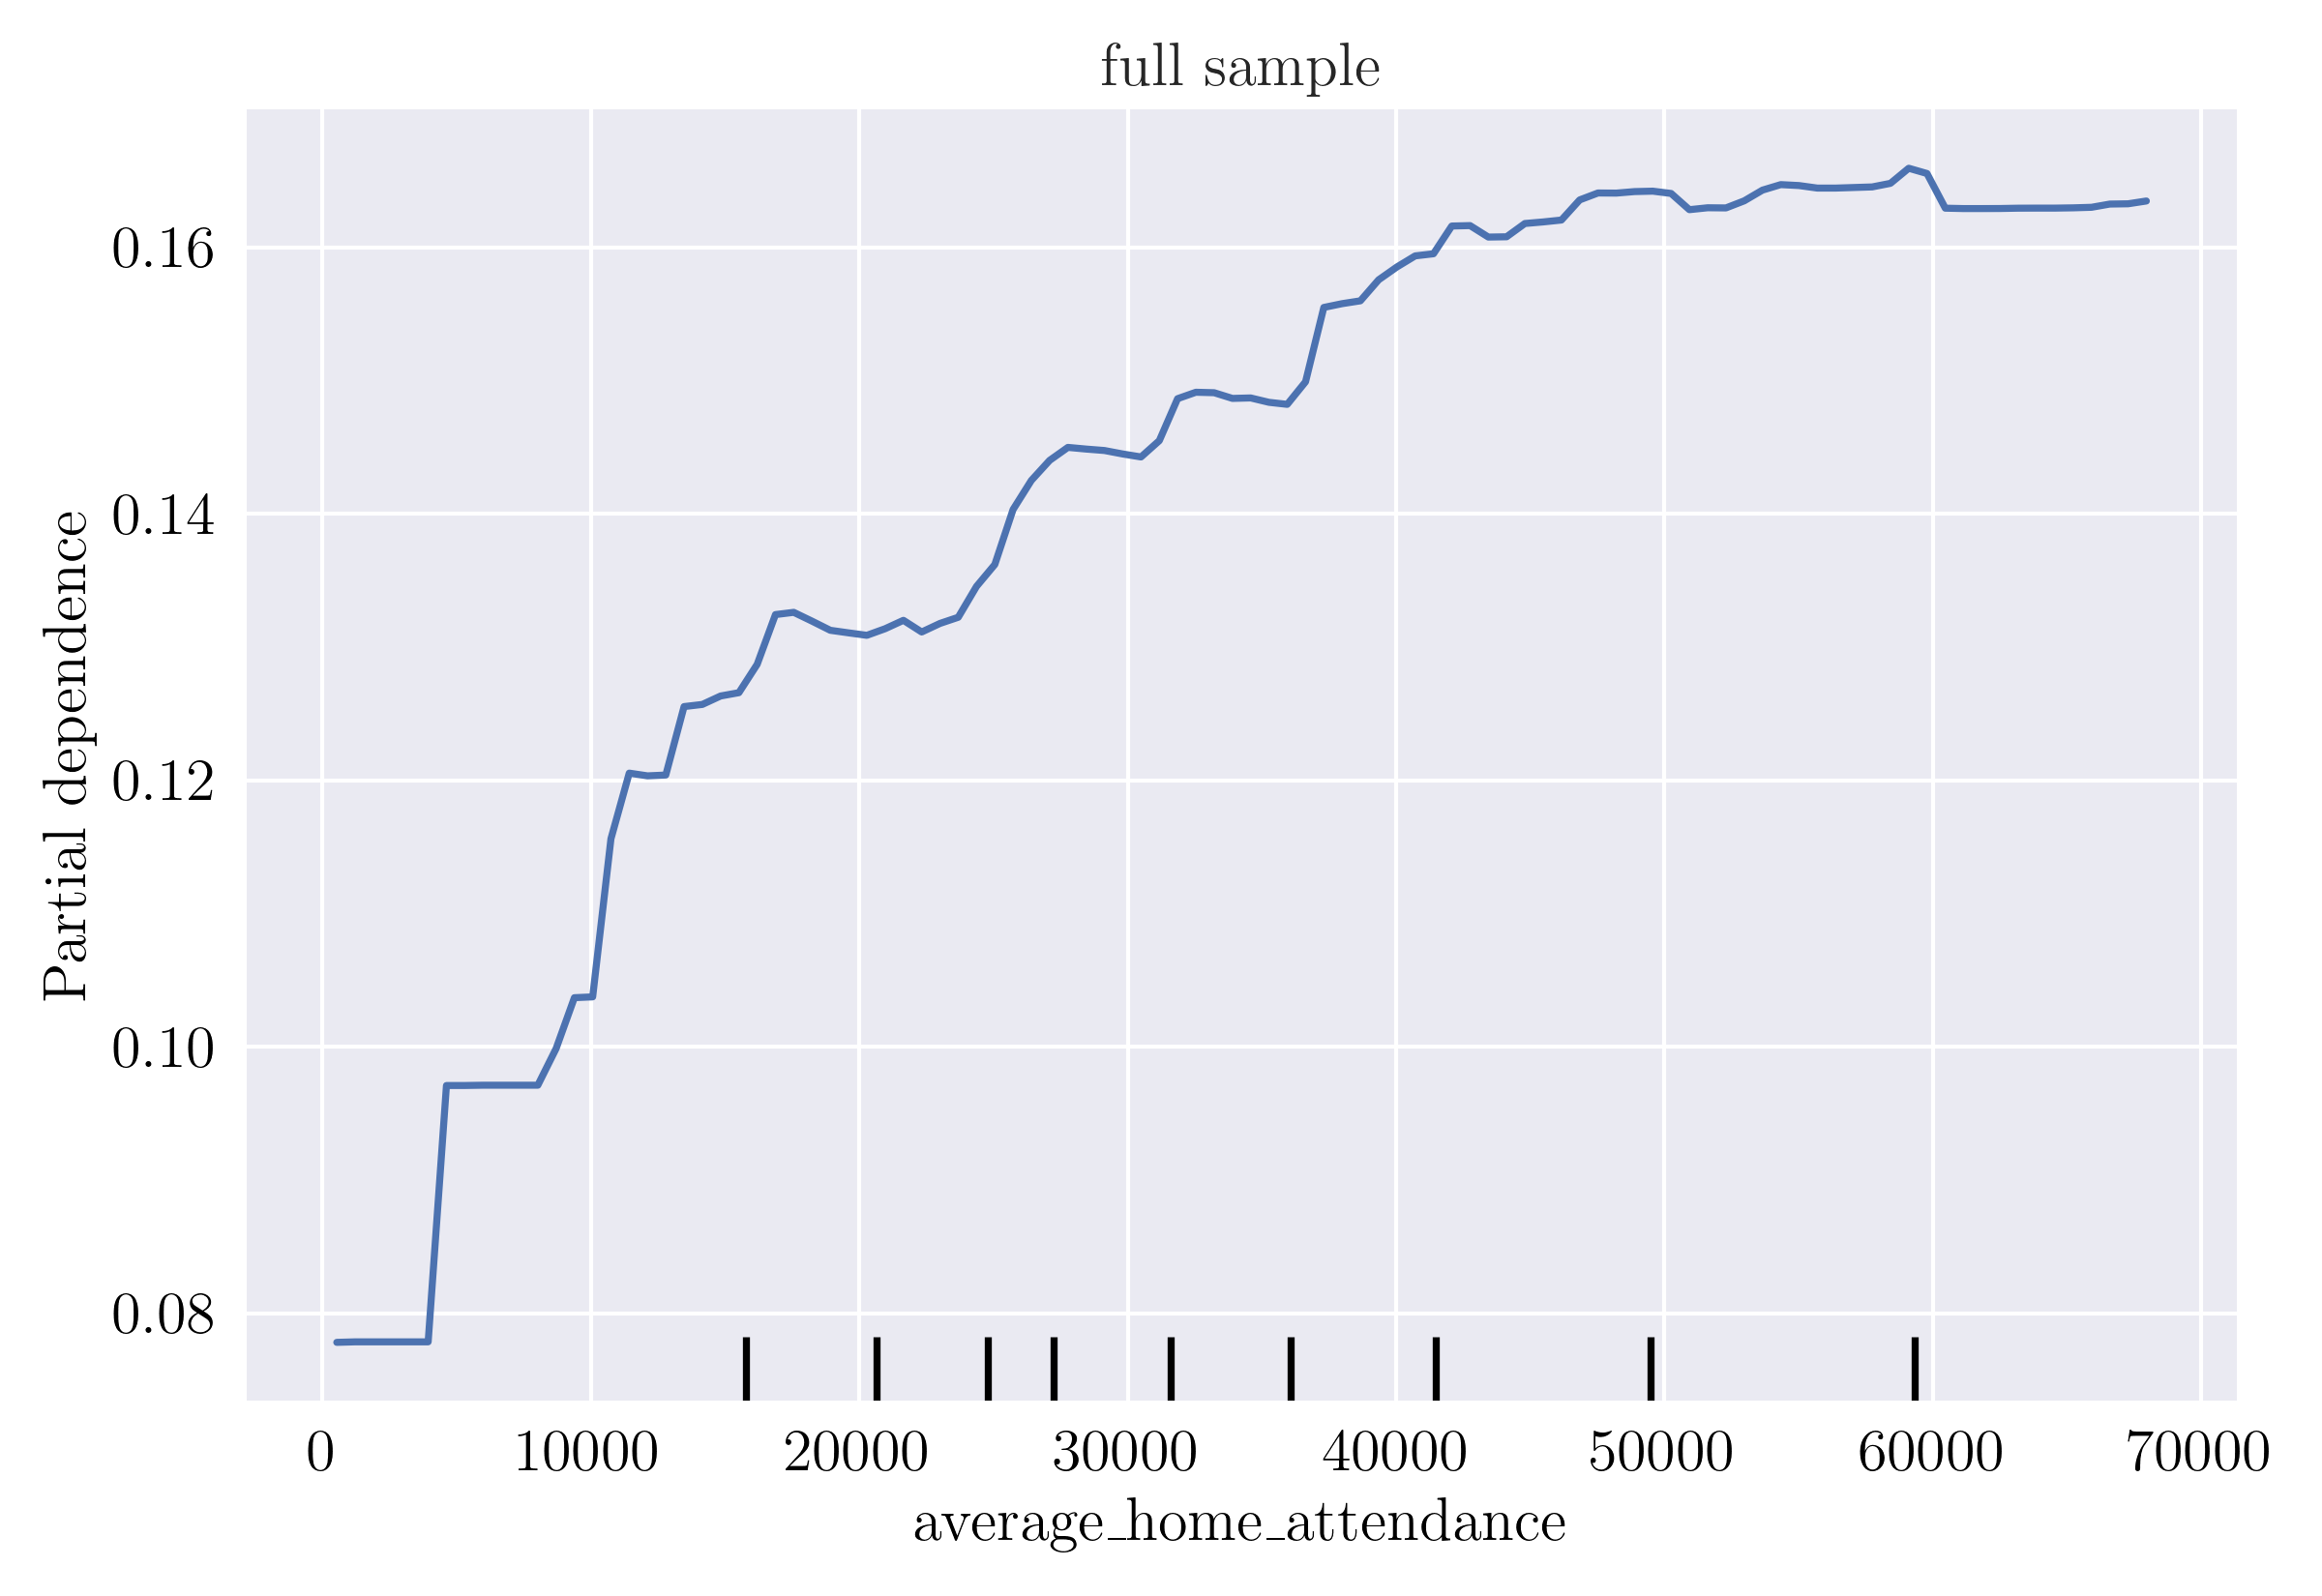
\includegraphics[width=0.49\linewidth]{attachments/machine-learning/pd_aha_rf_full_sample.png}
    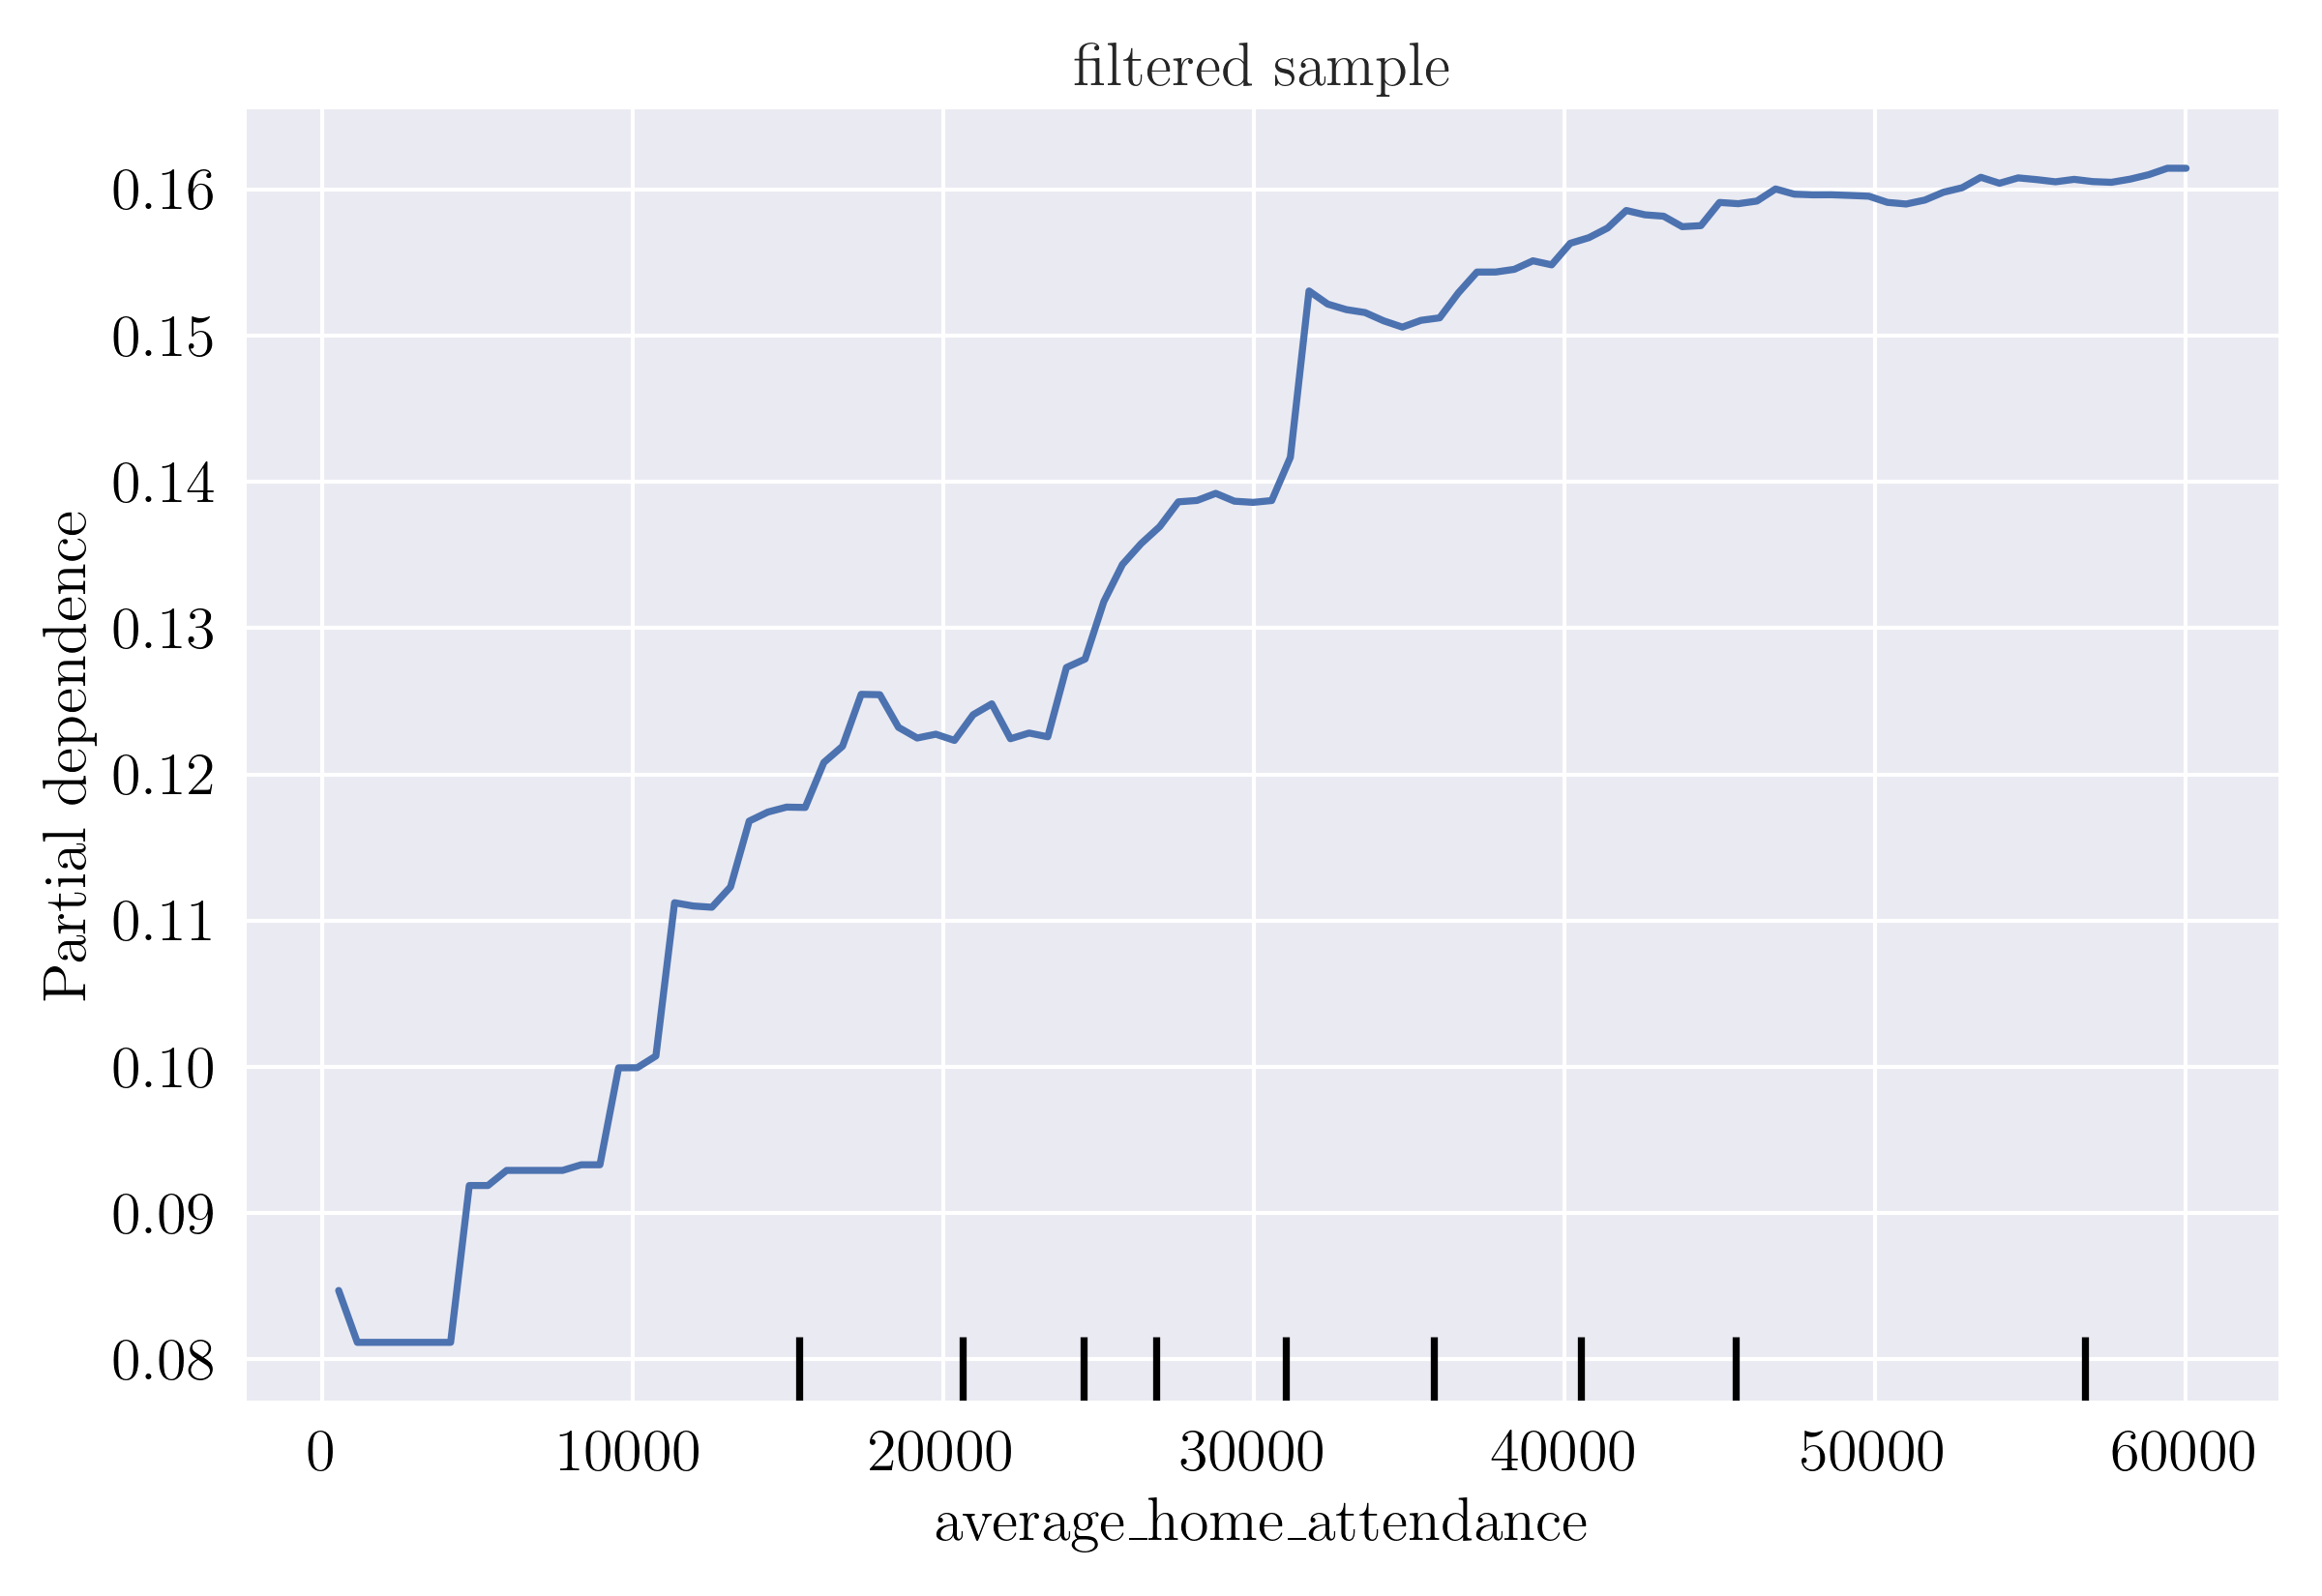
\includegraphics[width=0.49\linewidth]{attachments/machine-learning/pd_aha_rf_filtered_sample.png}
    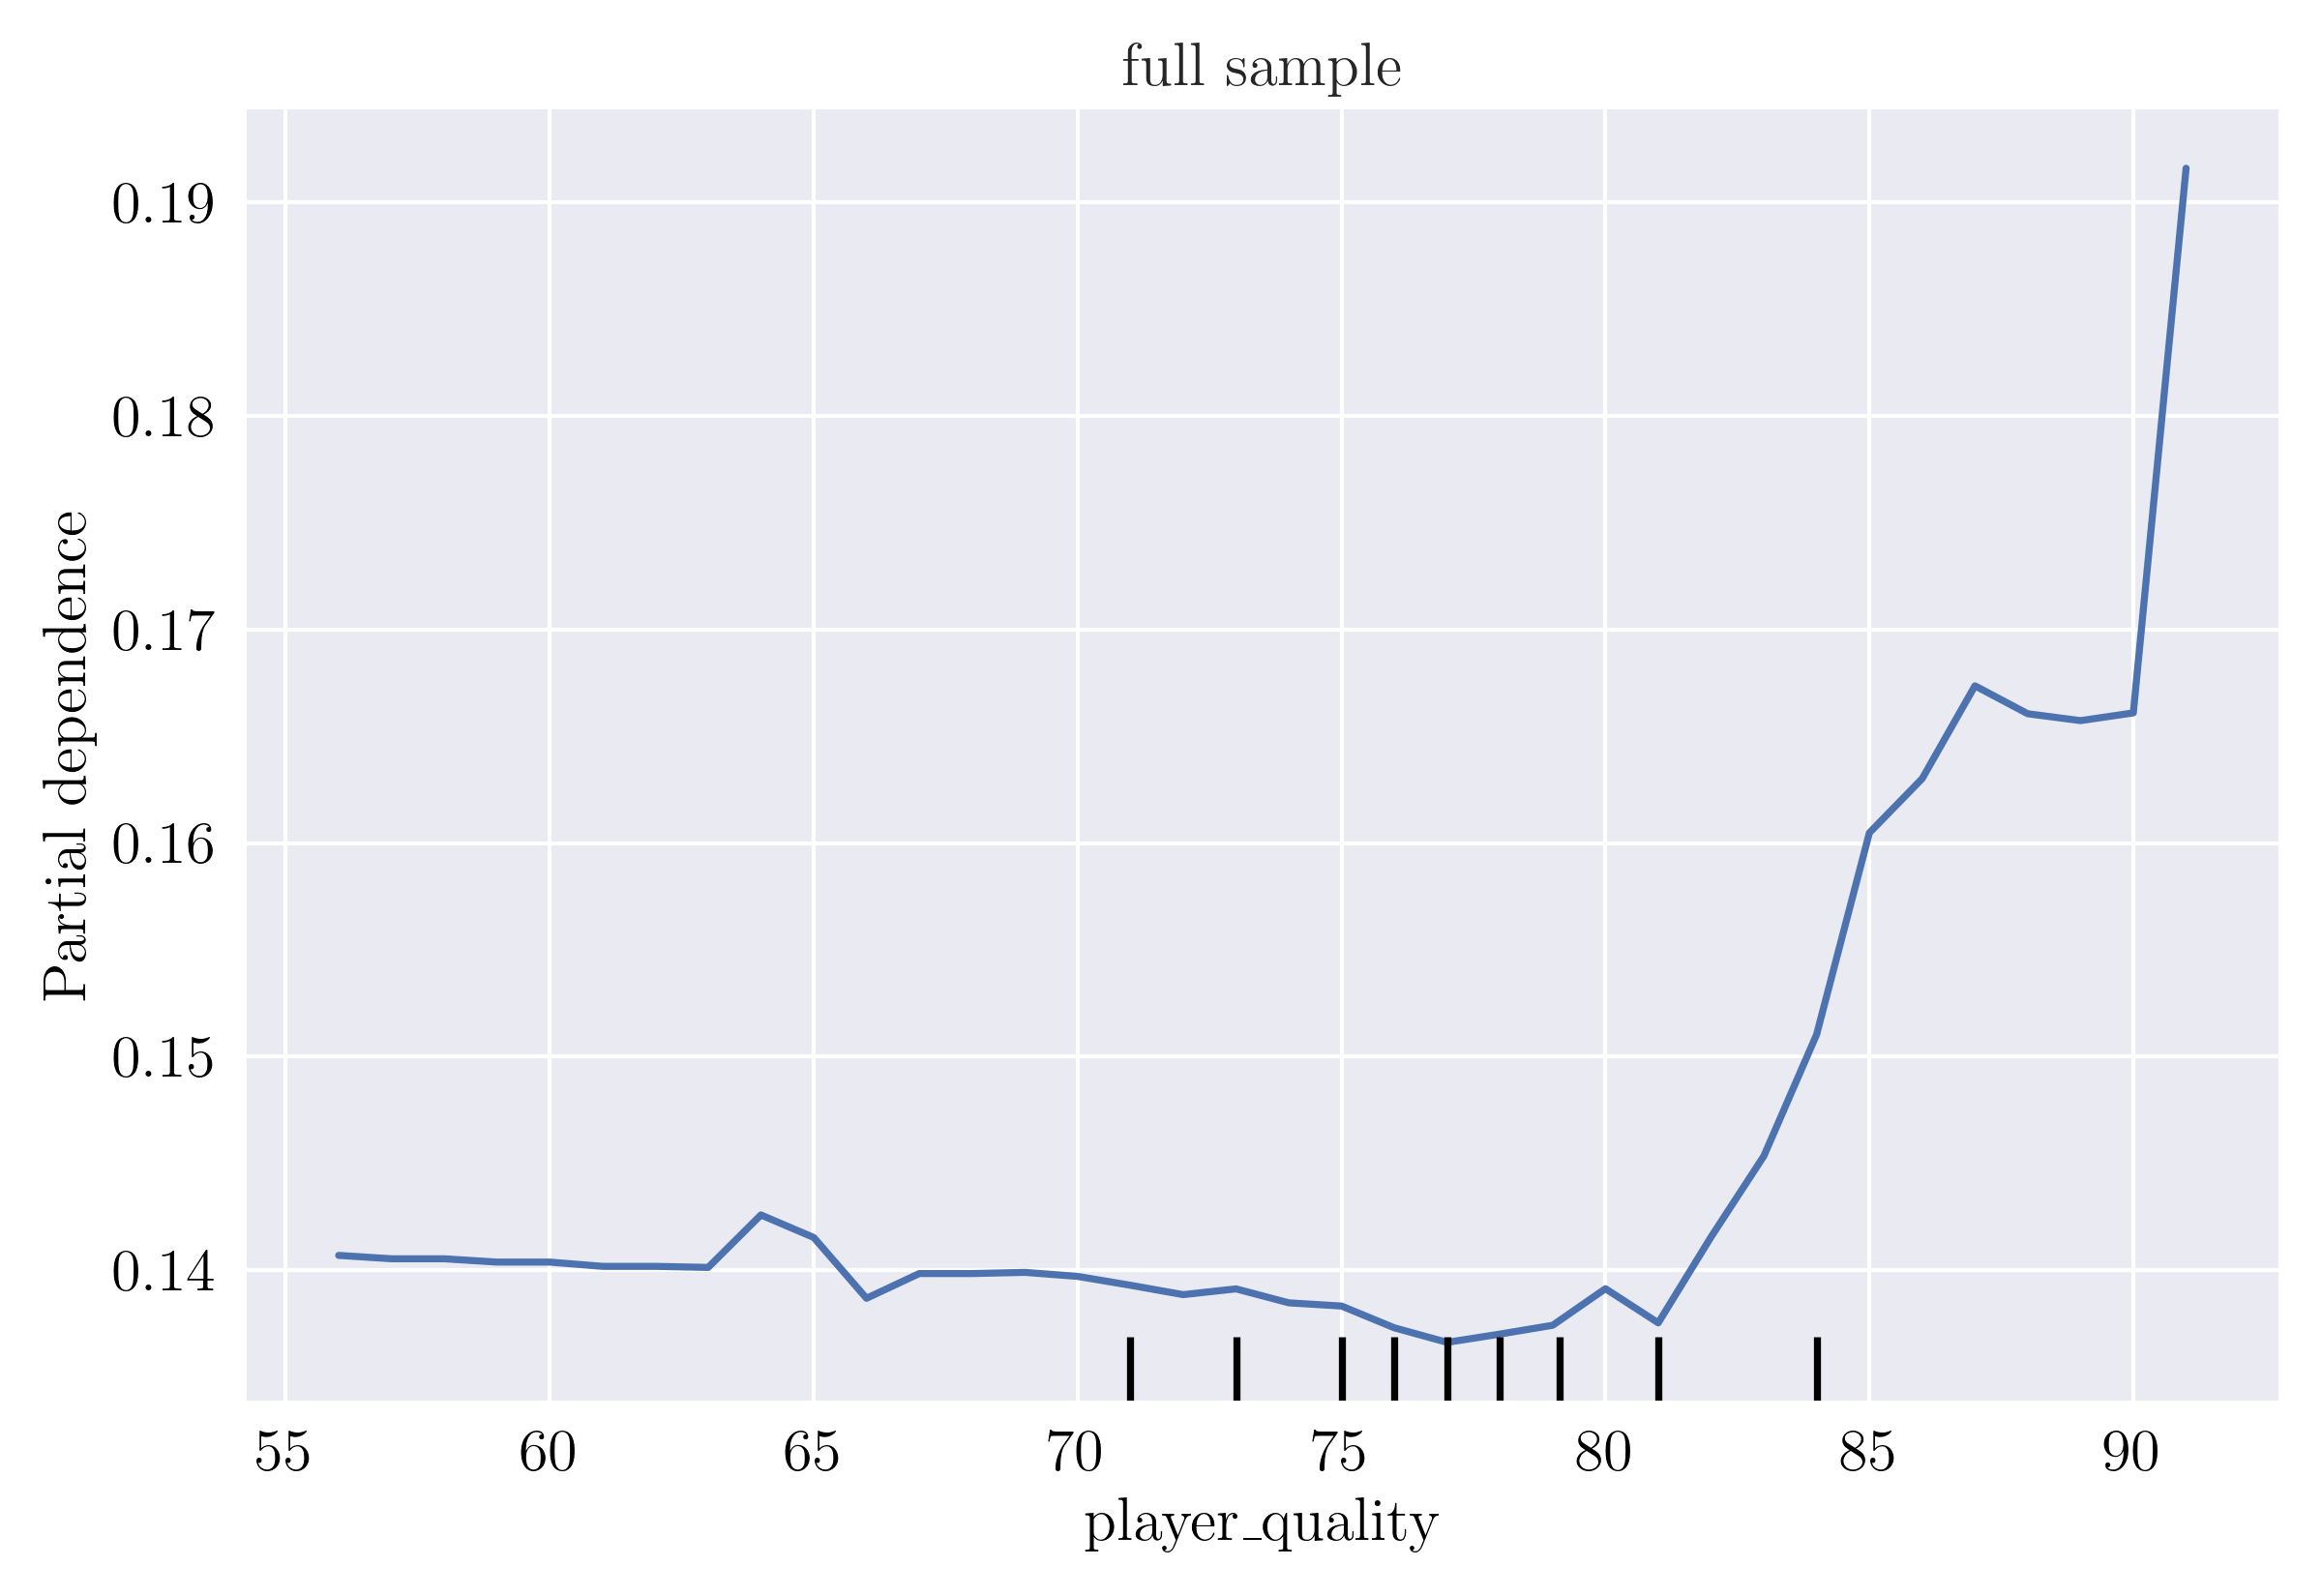
\includegraphics[width=0.49\linewidth]{attachments/machine-learning/pd_pr_rf_full_sample.png}
    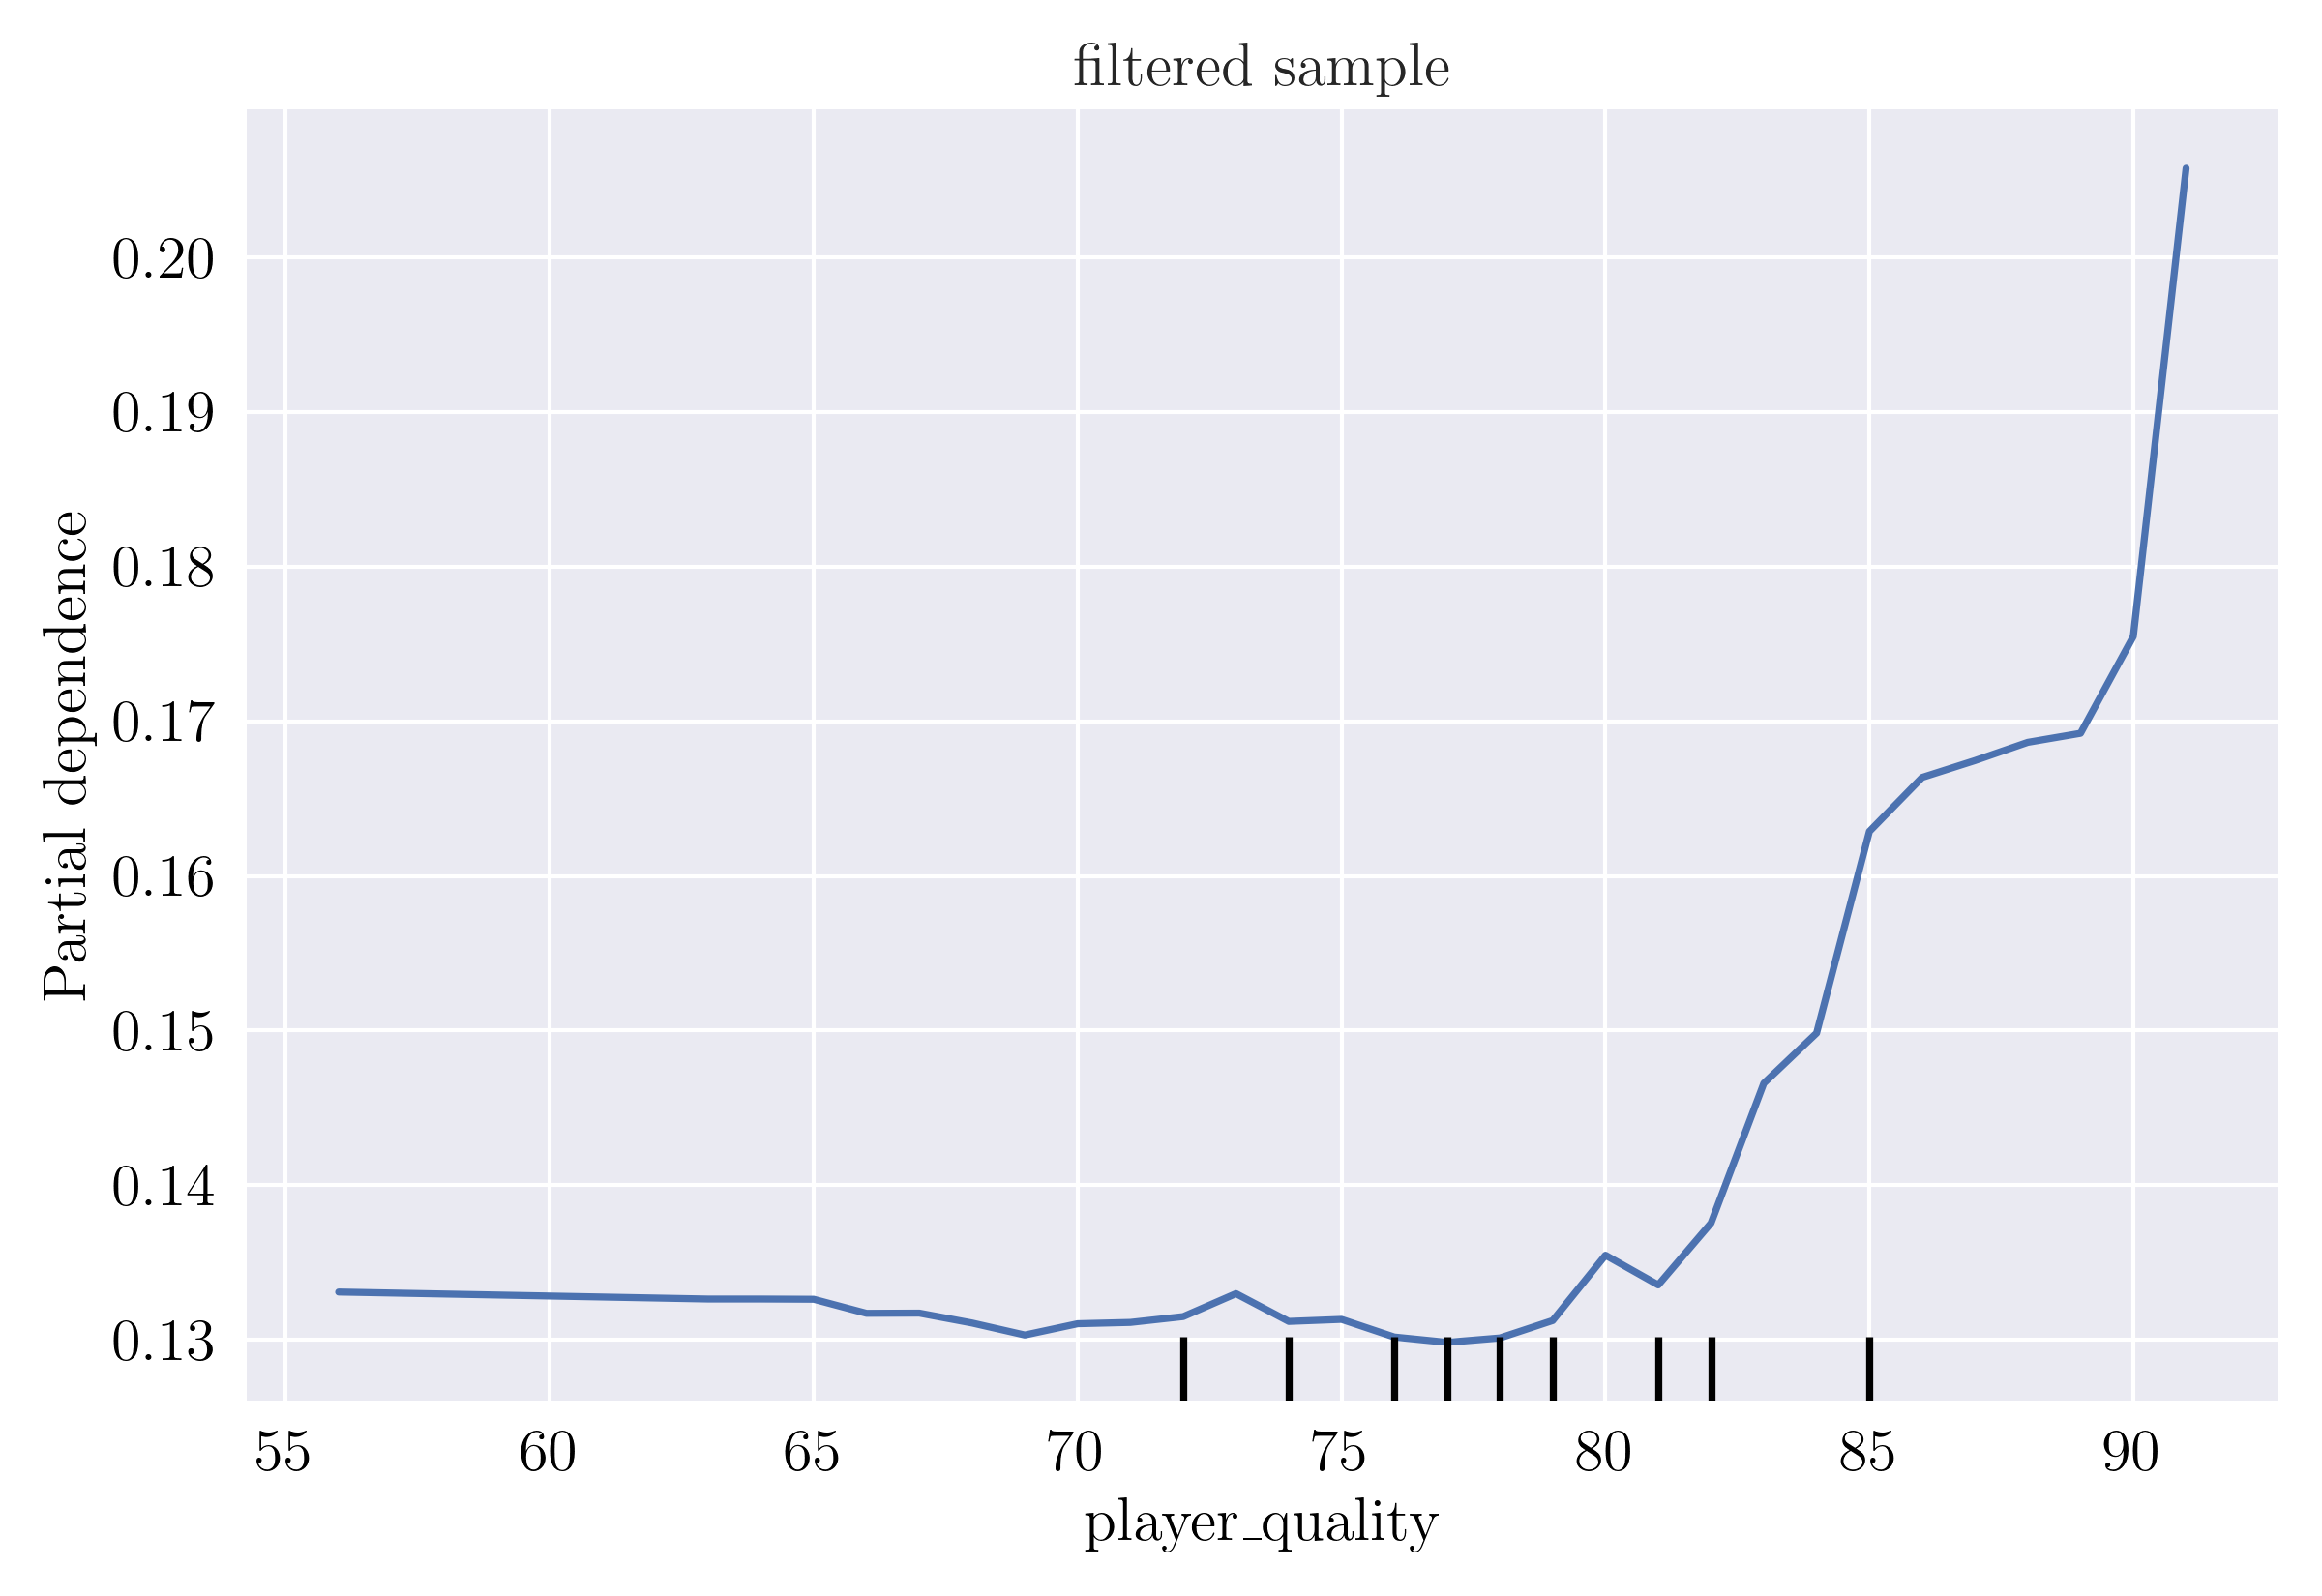
\includegraphics[width=0.49\linewidth]{attachments/machine-learning/pd_pr_rf_filtered_sample.png}
    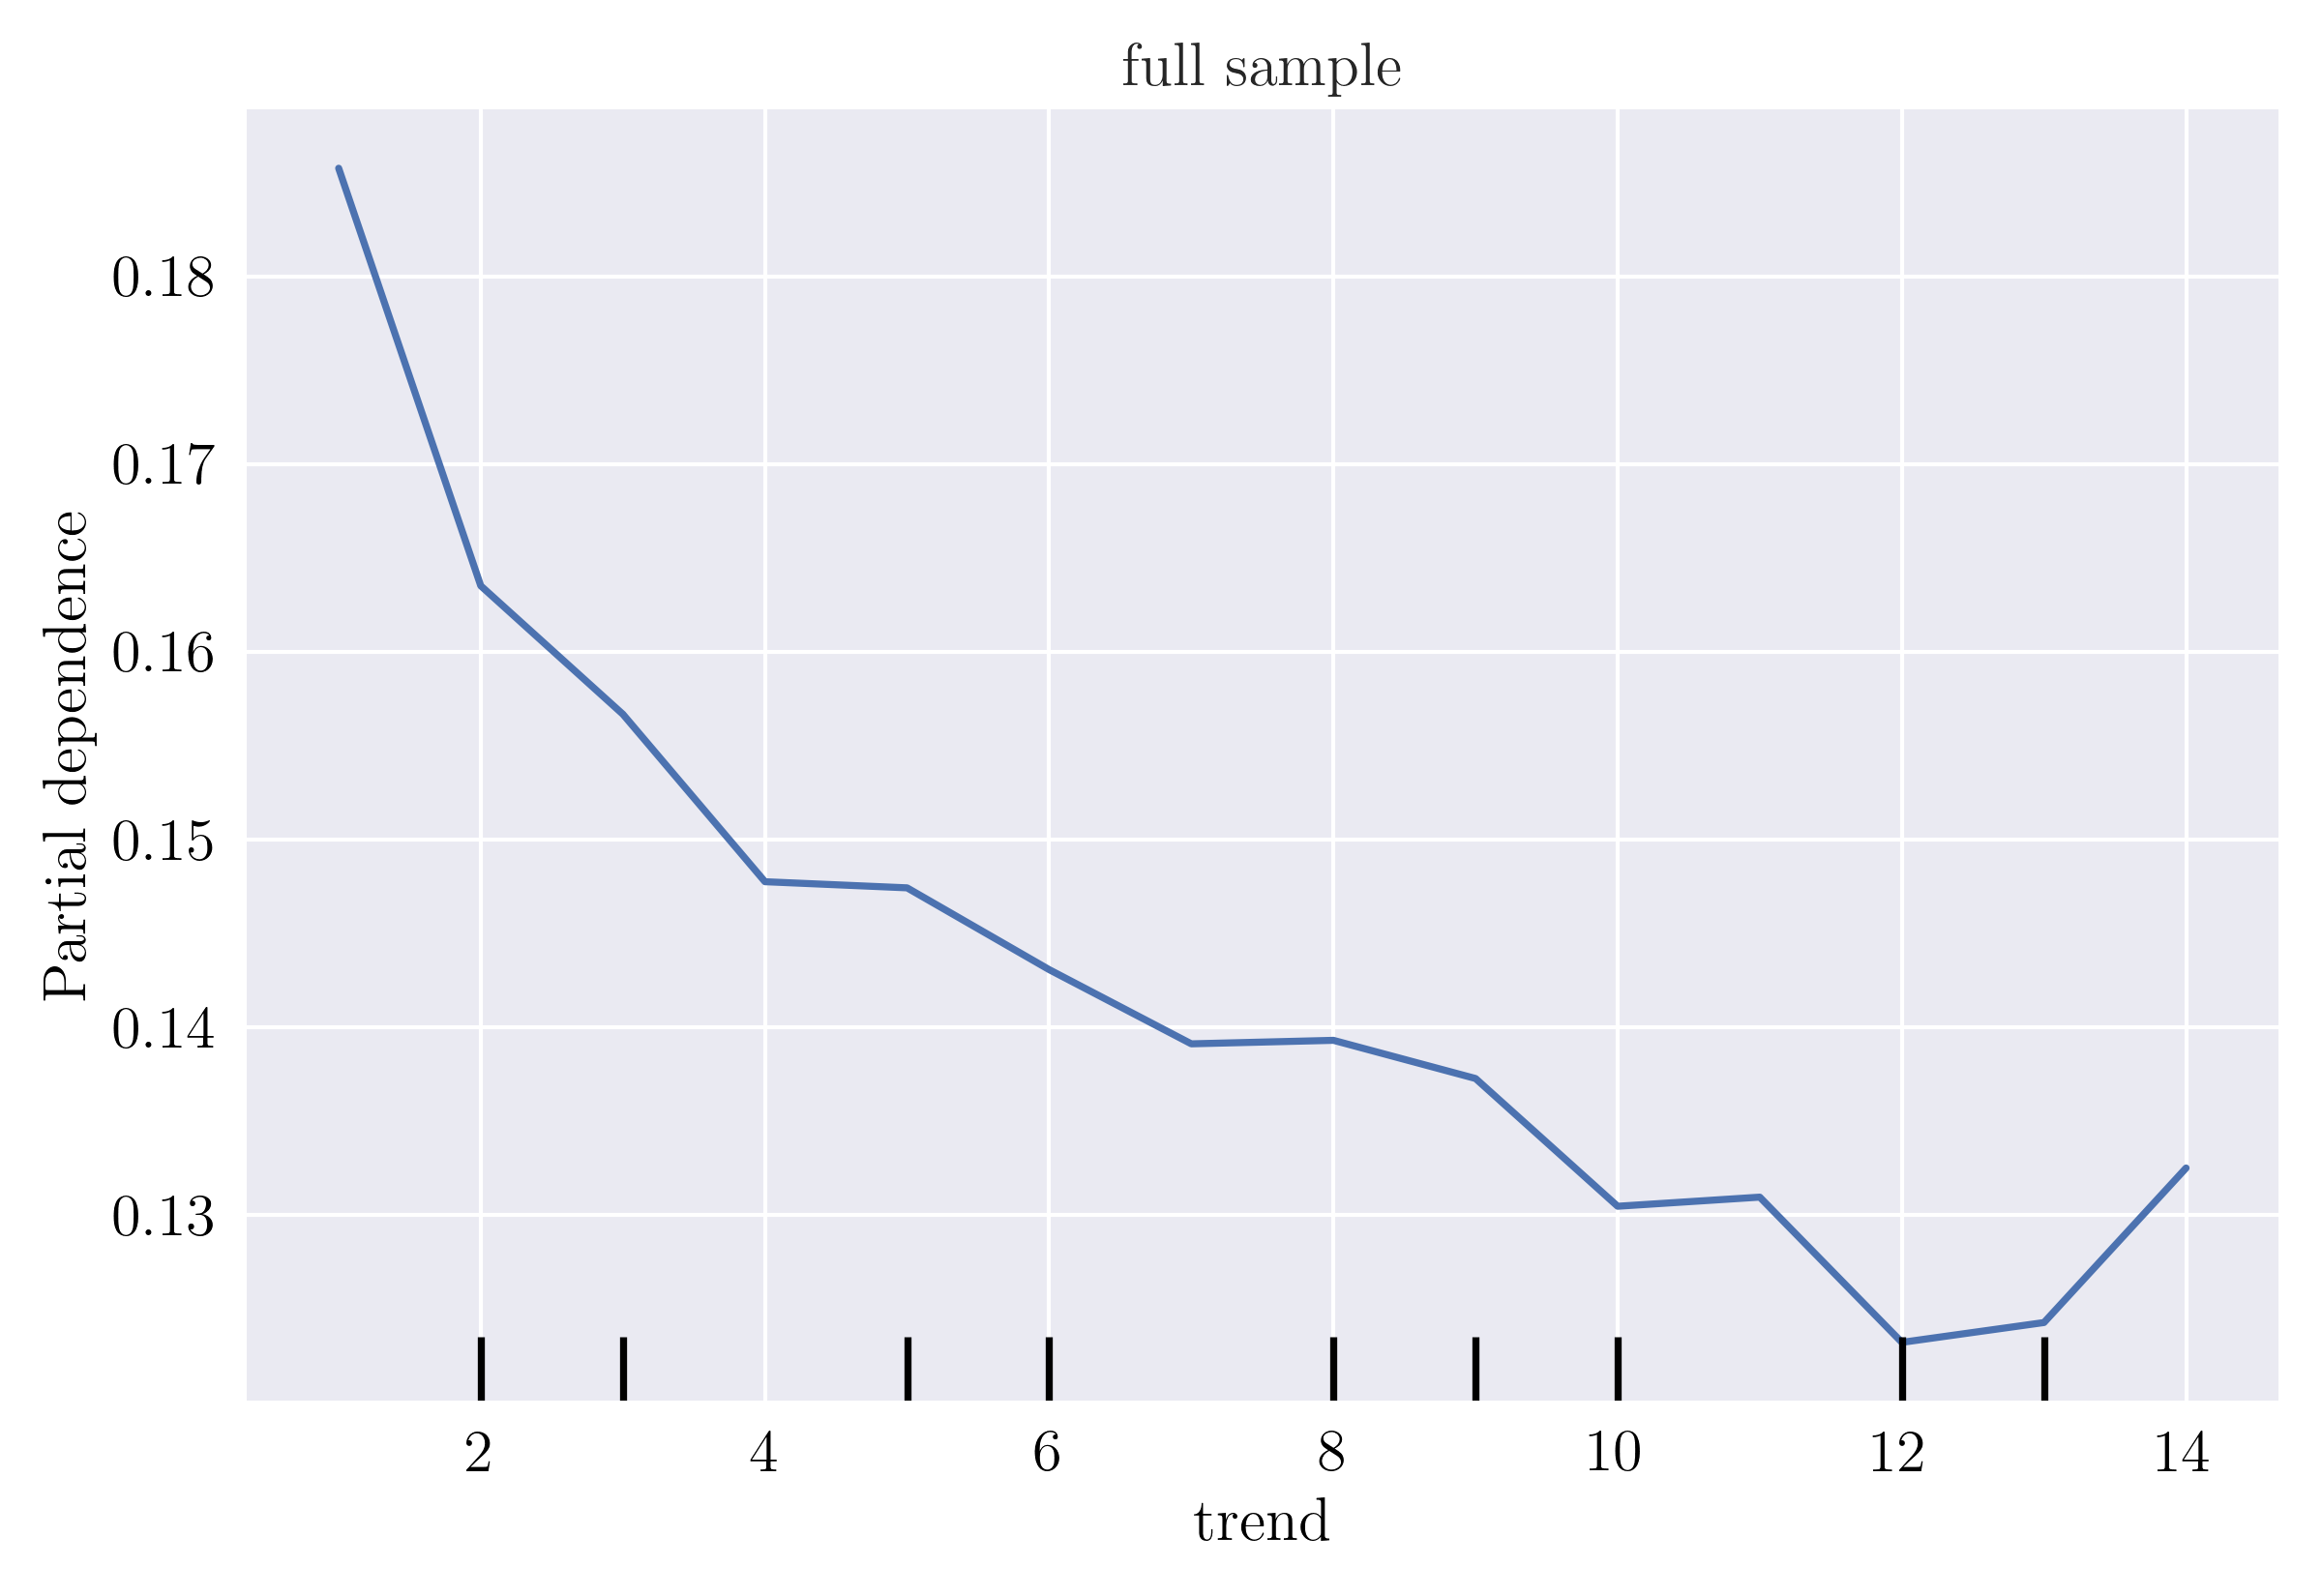
\includegraphics[width=0.49\linewidth]{attachments/machine-learning/pd_trend_rf_full_sample.png}
    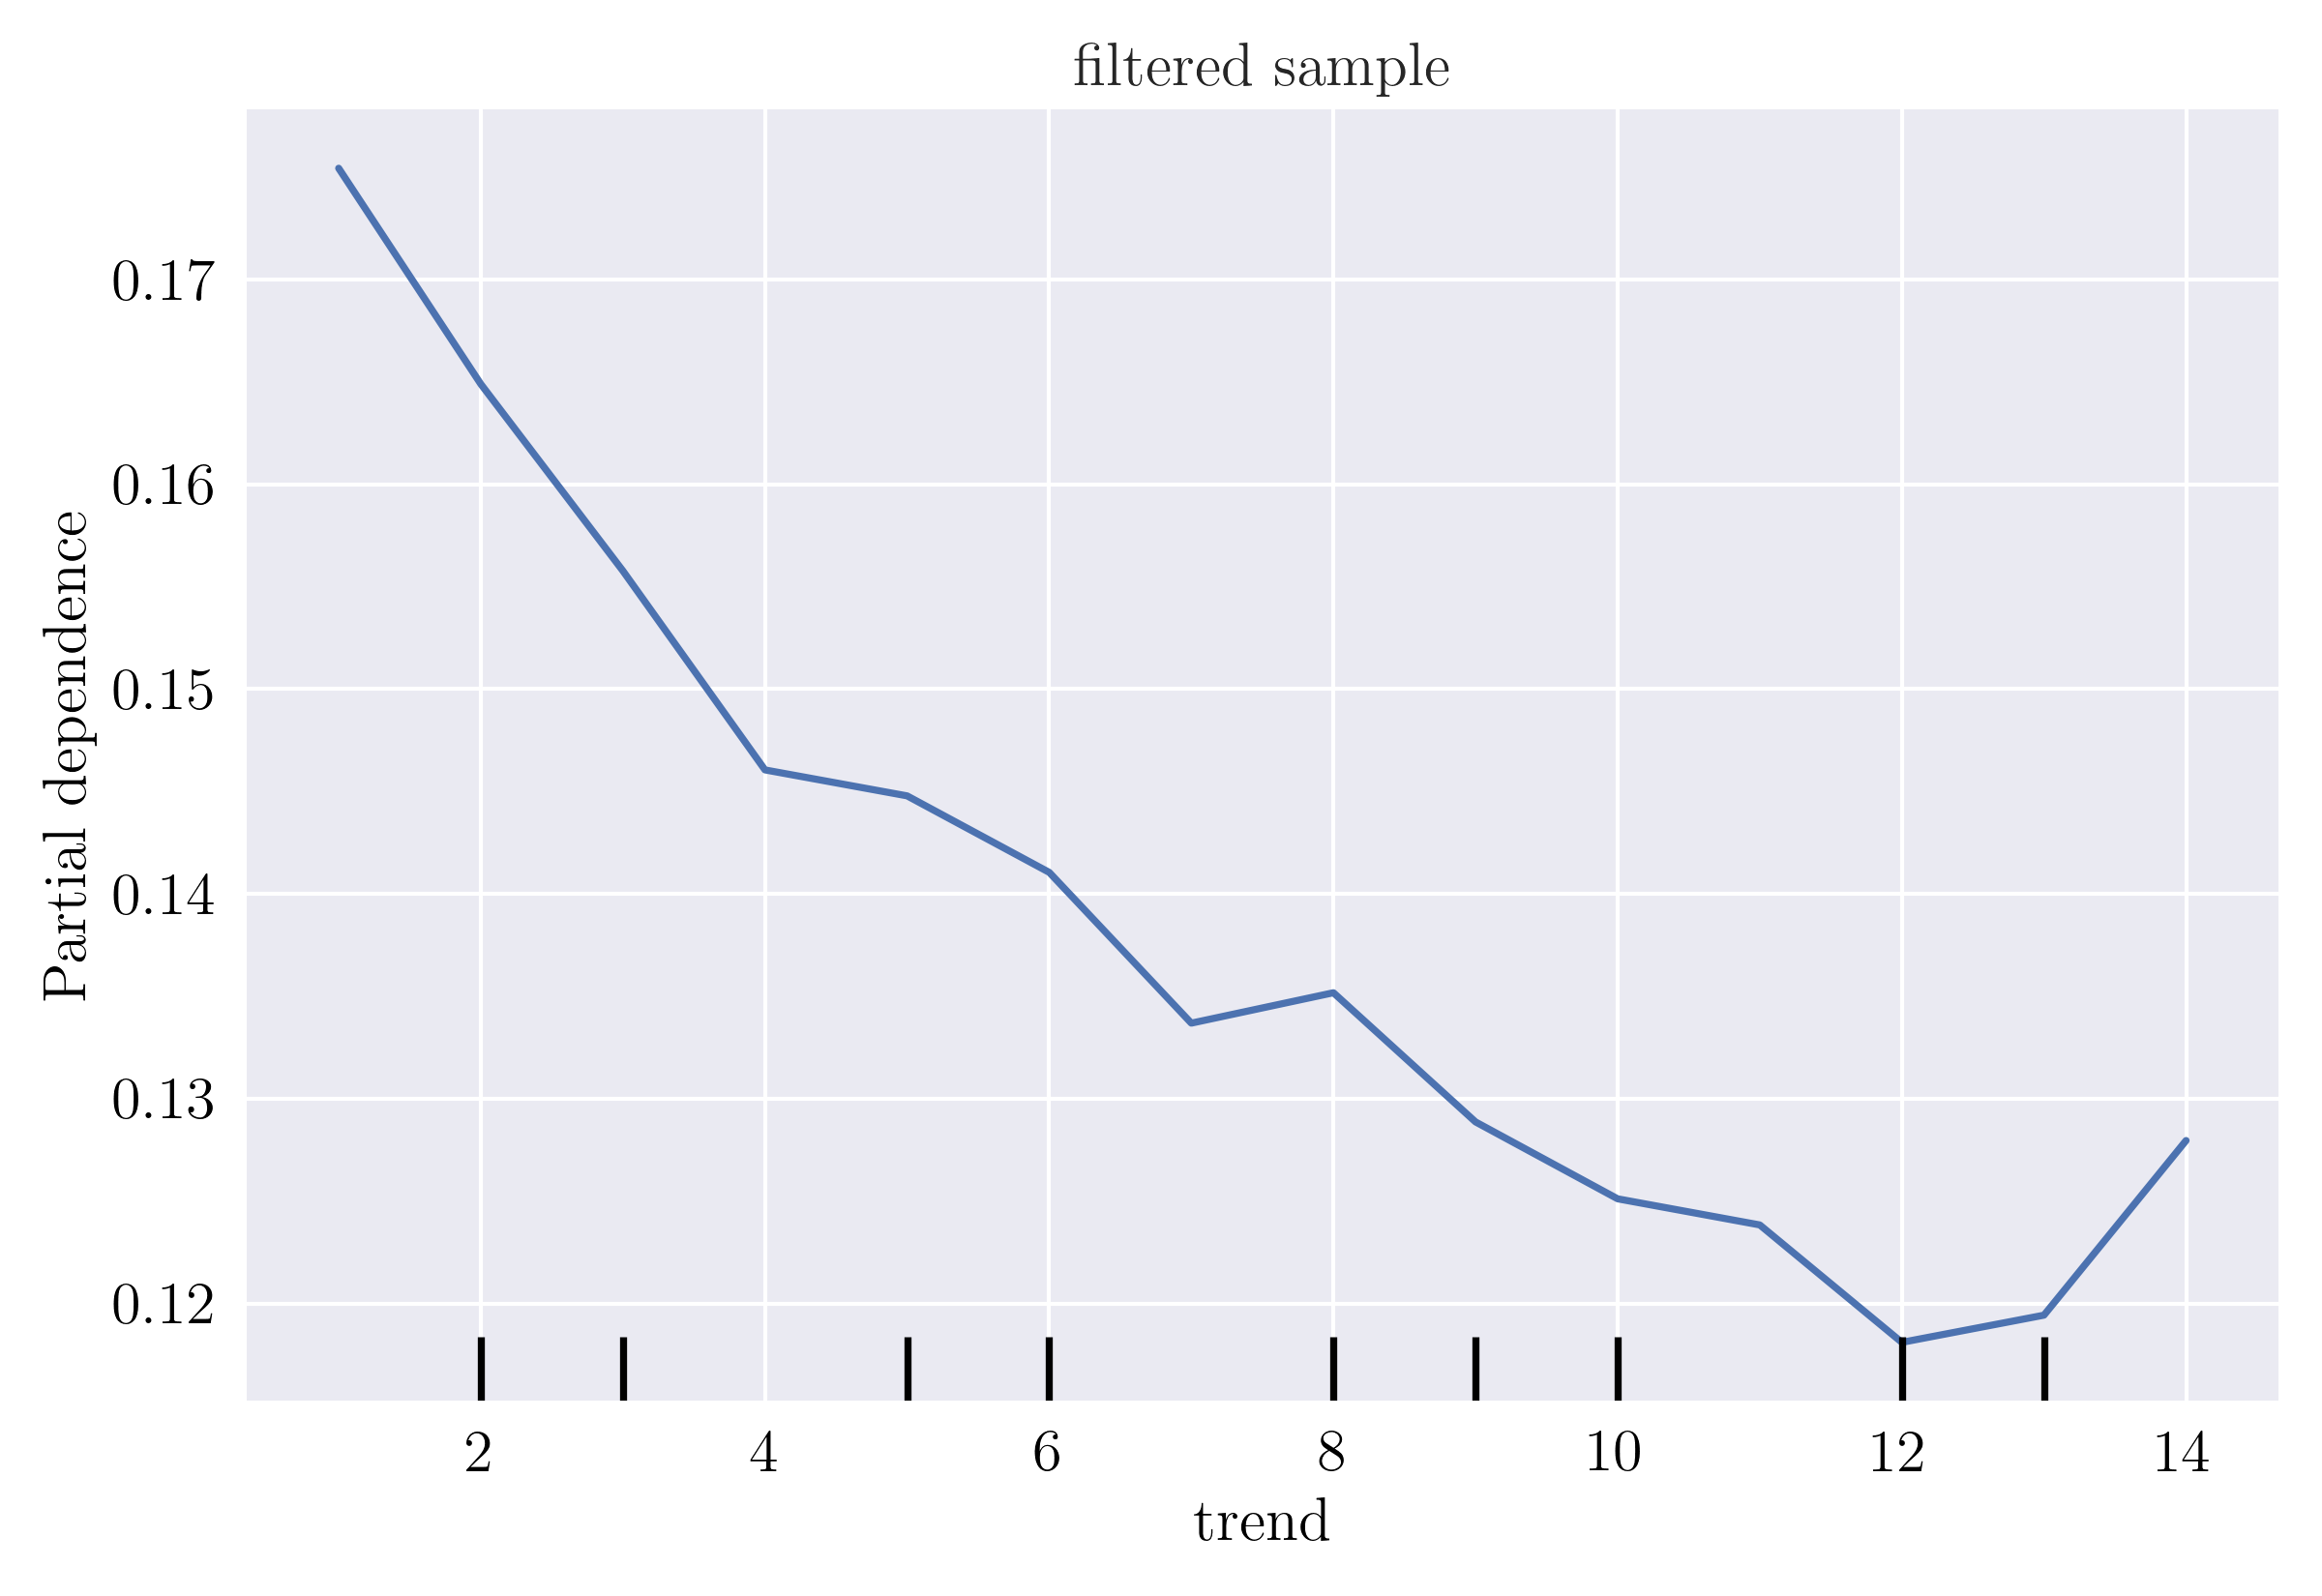
\includegraphics[width=0.49\linewidth]{attachments/machine-learning/pd_trend_rf_filtered_sample.png}
    \caption{Partial dependence plots for the effect of average home attendance, player quality and trend on the home advantage a player enjoys}
    \label{fig:pd_plots_1}
\end{figure}

\begin{figure}
    \centering
    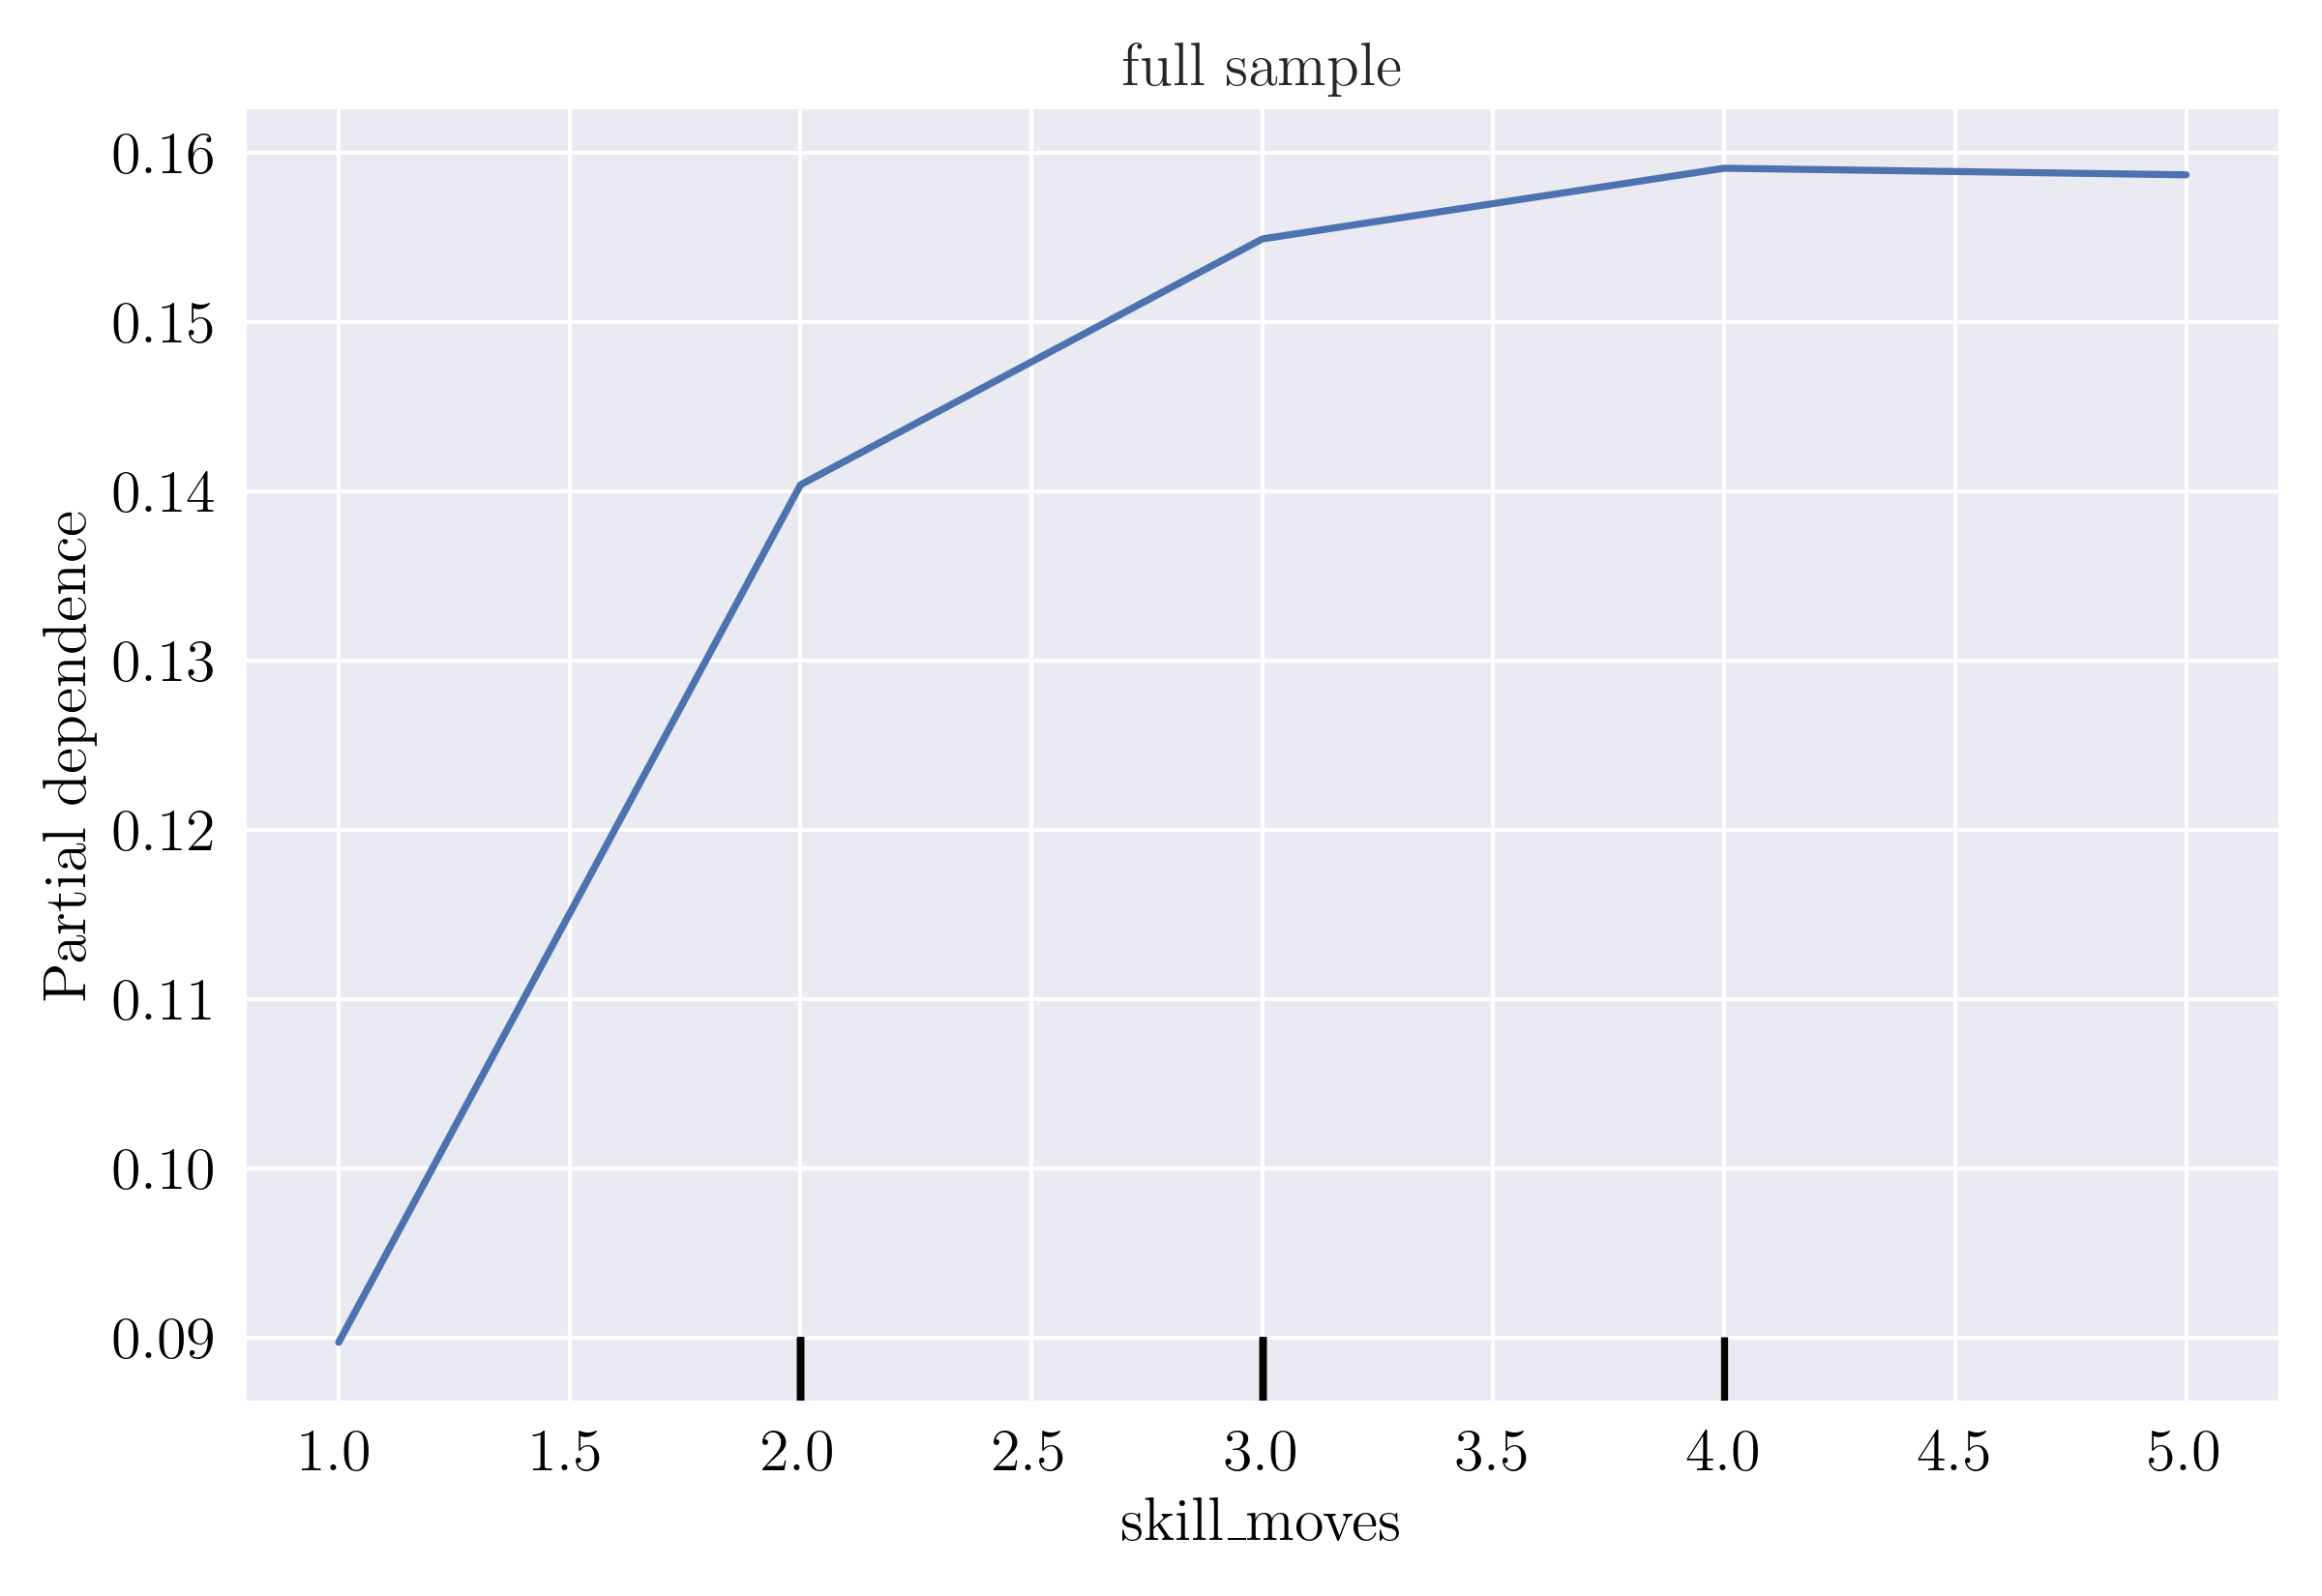
\includegraphics[width=0.49\linewidth]{attachments/machine-learning/pd_sm_rf_full_sample.png}
    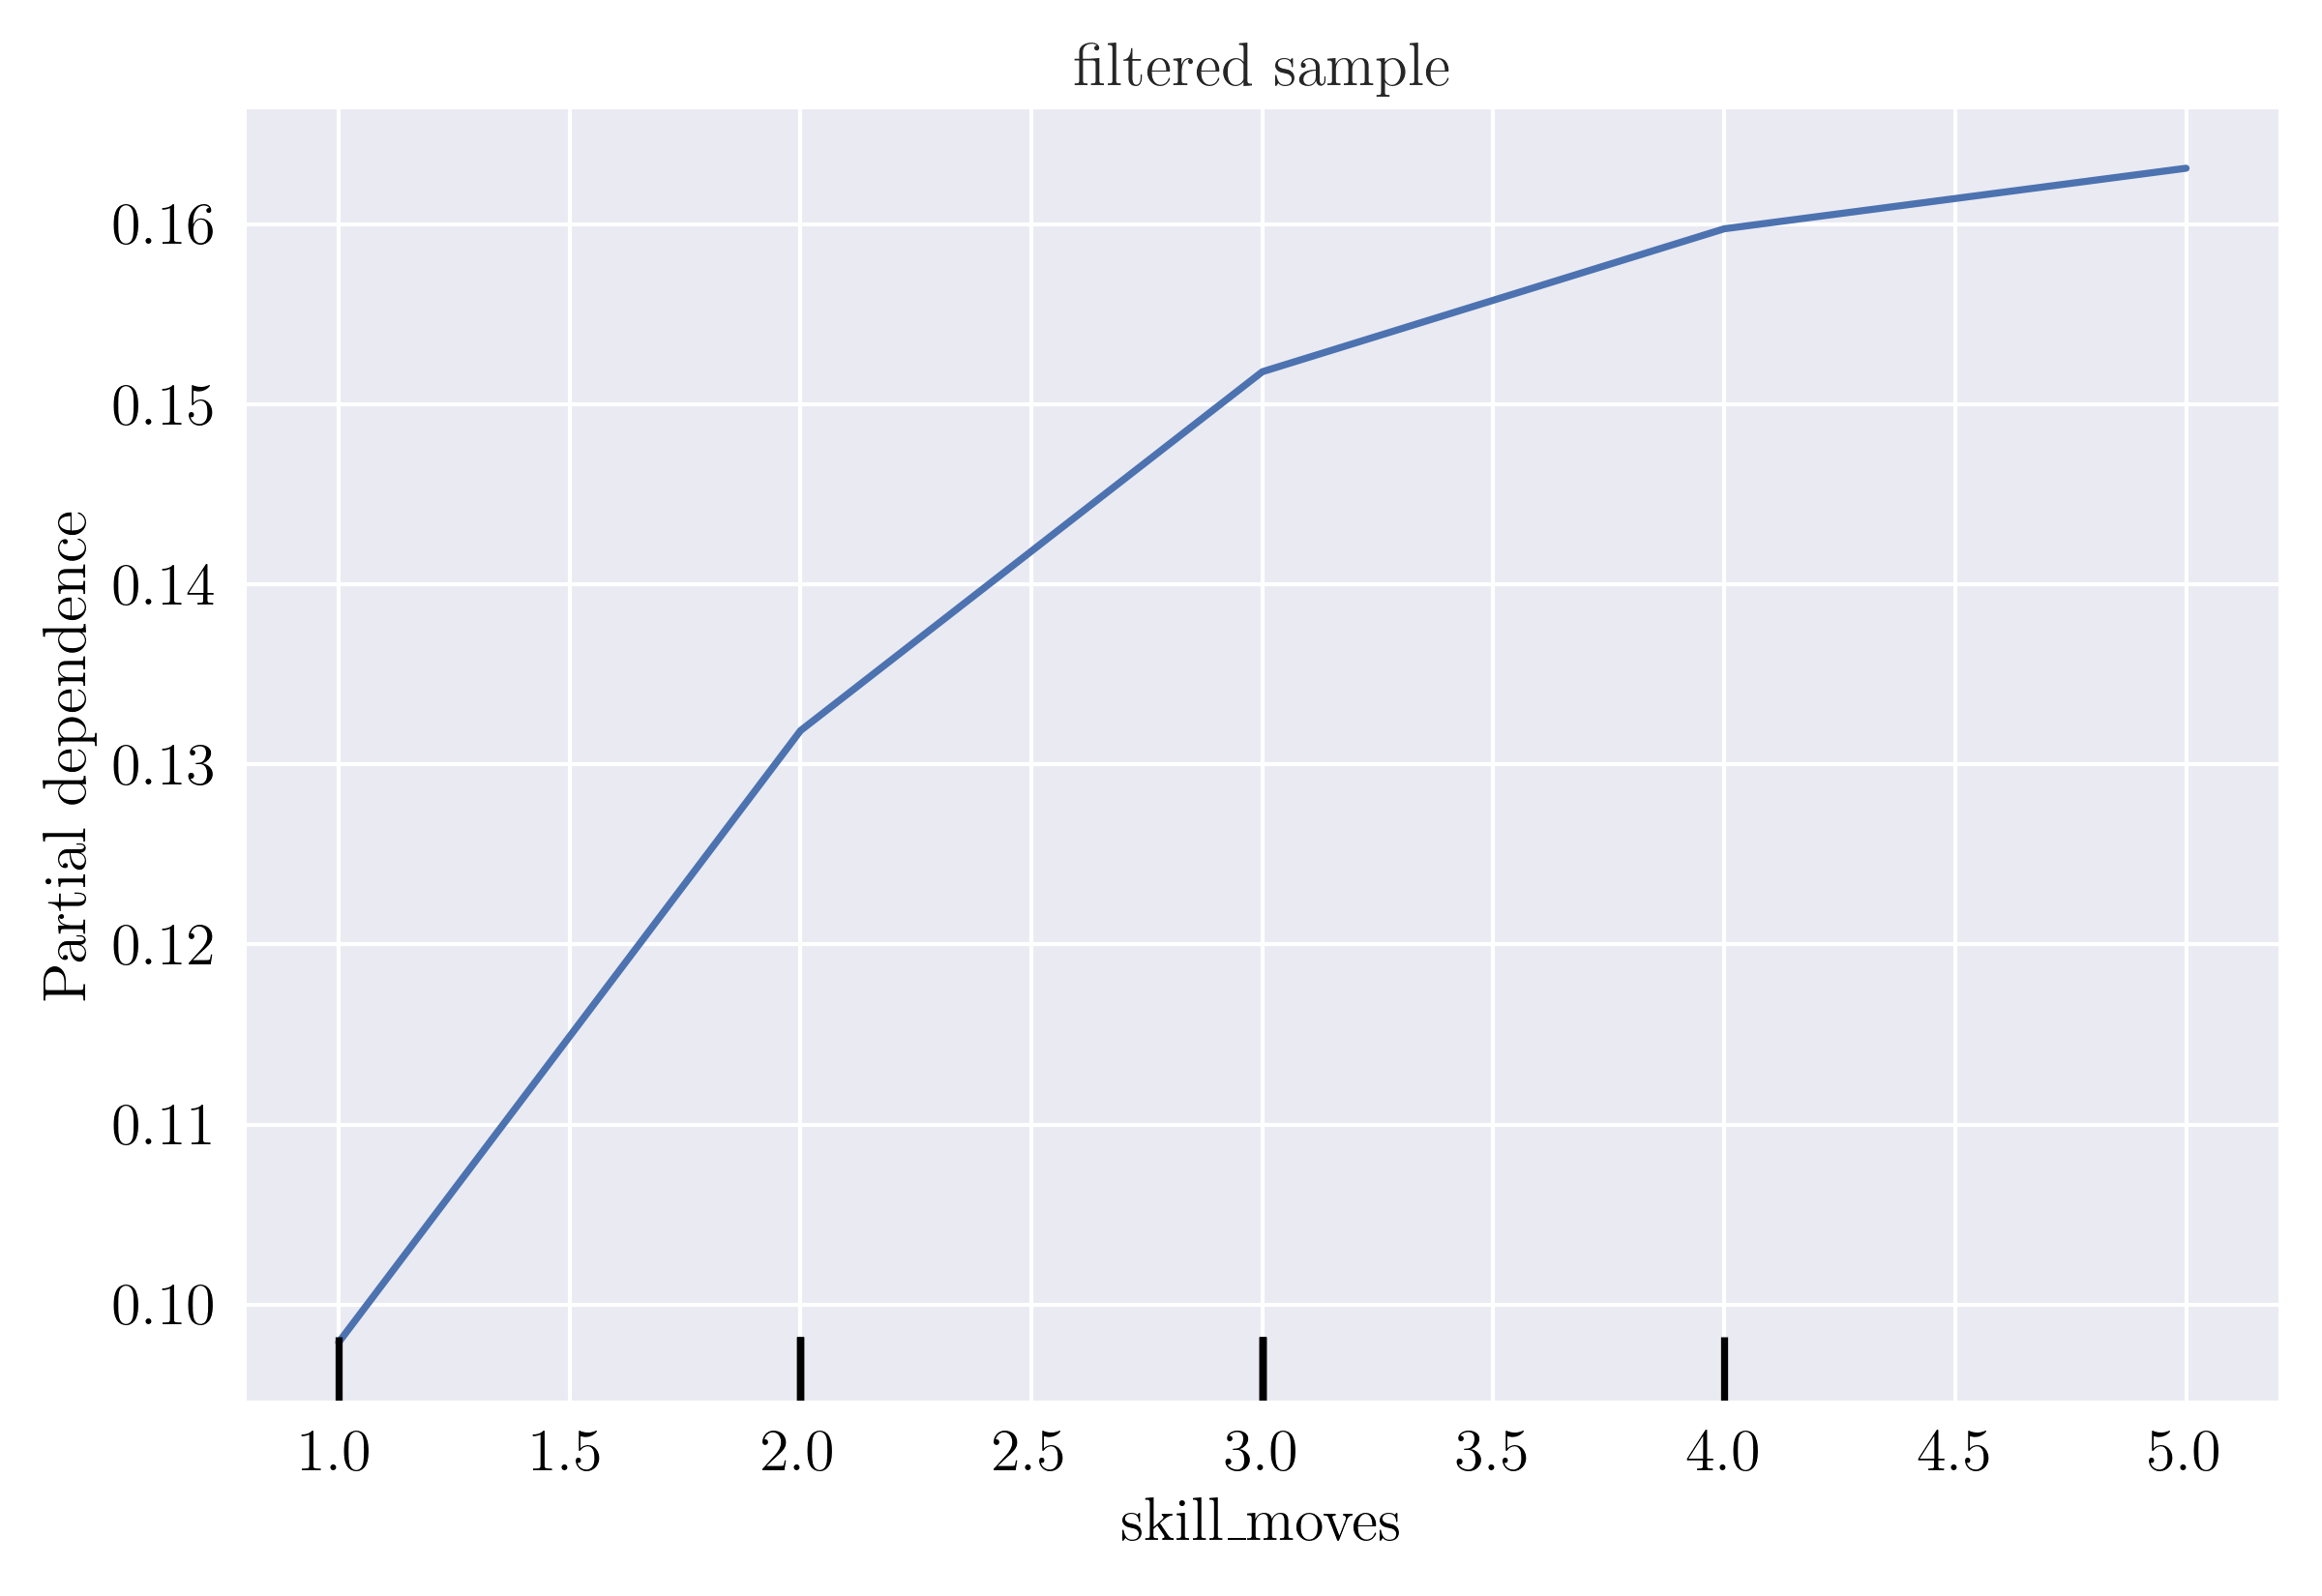
\includegraphics[width=0.49\linewidth]{attachments/machine-learning/pd_sm_rf_filtered_sample.png}
    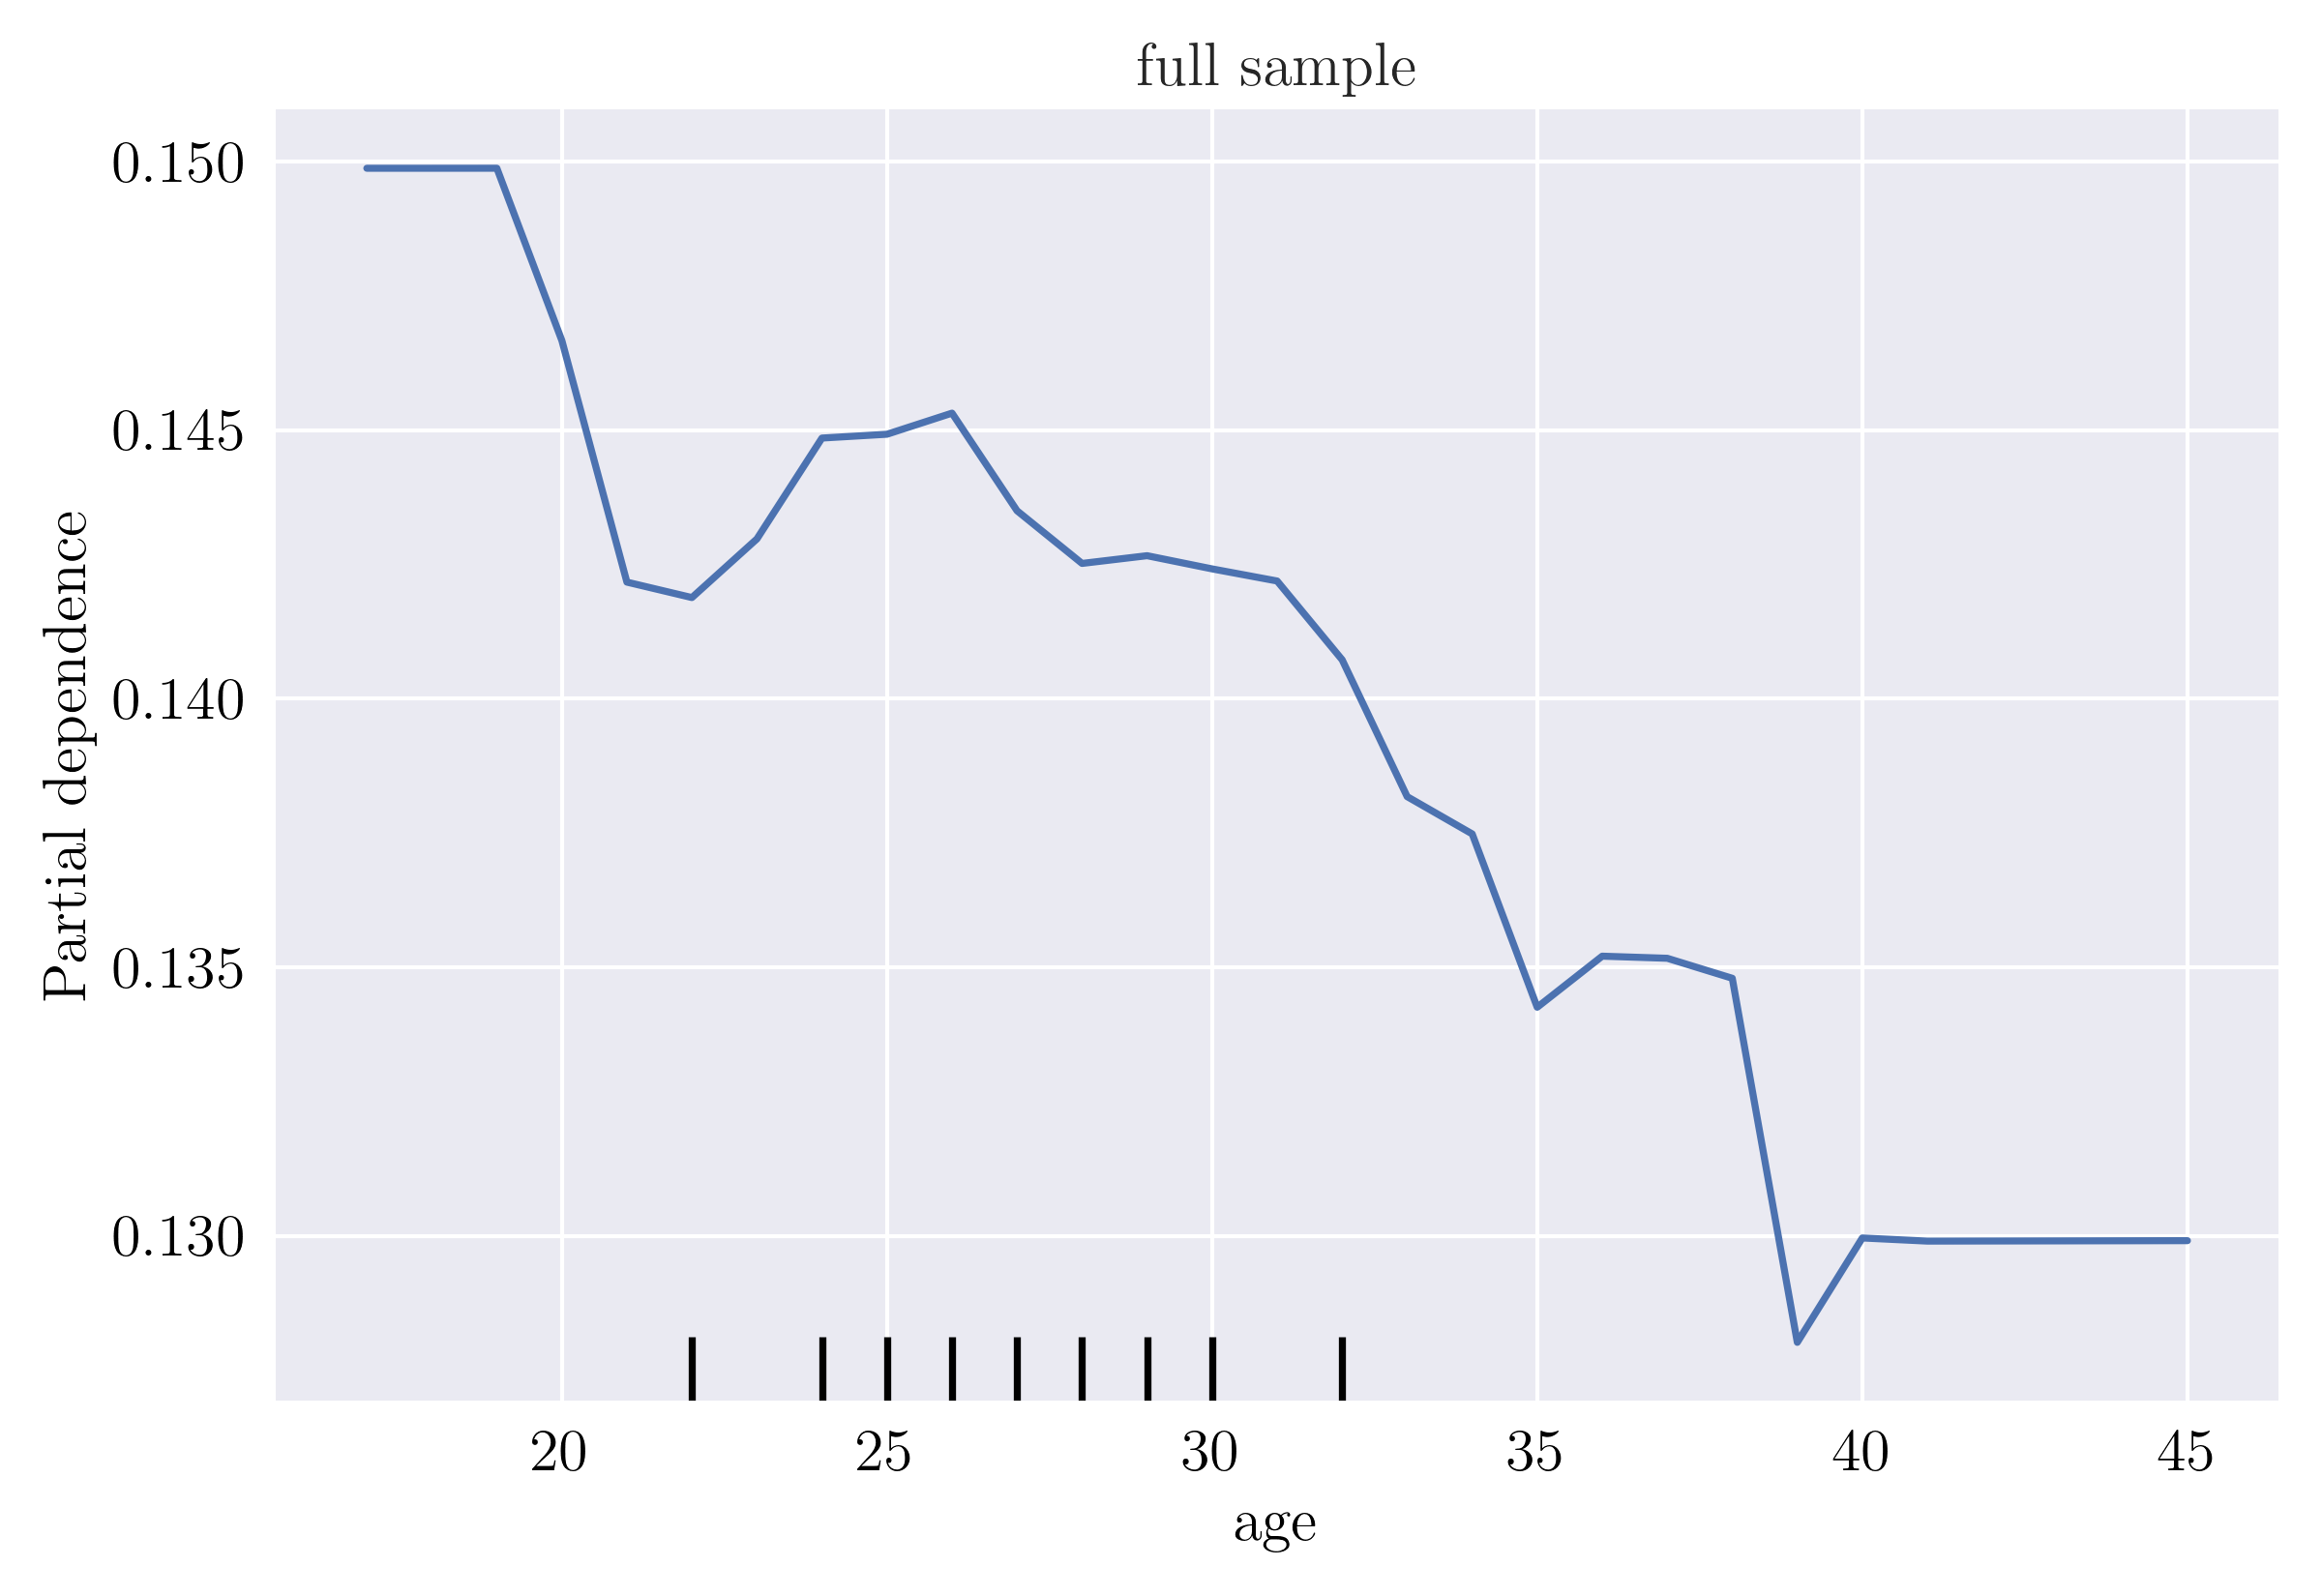
\includegraphics[width=0.49\linewidth]{attachments/machine-learning/pd_age_rf_full_sample.png}
    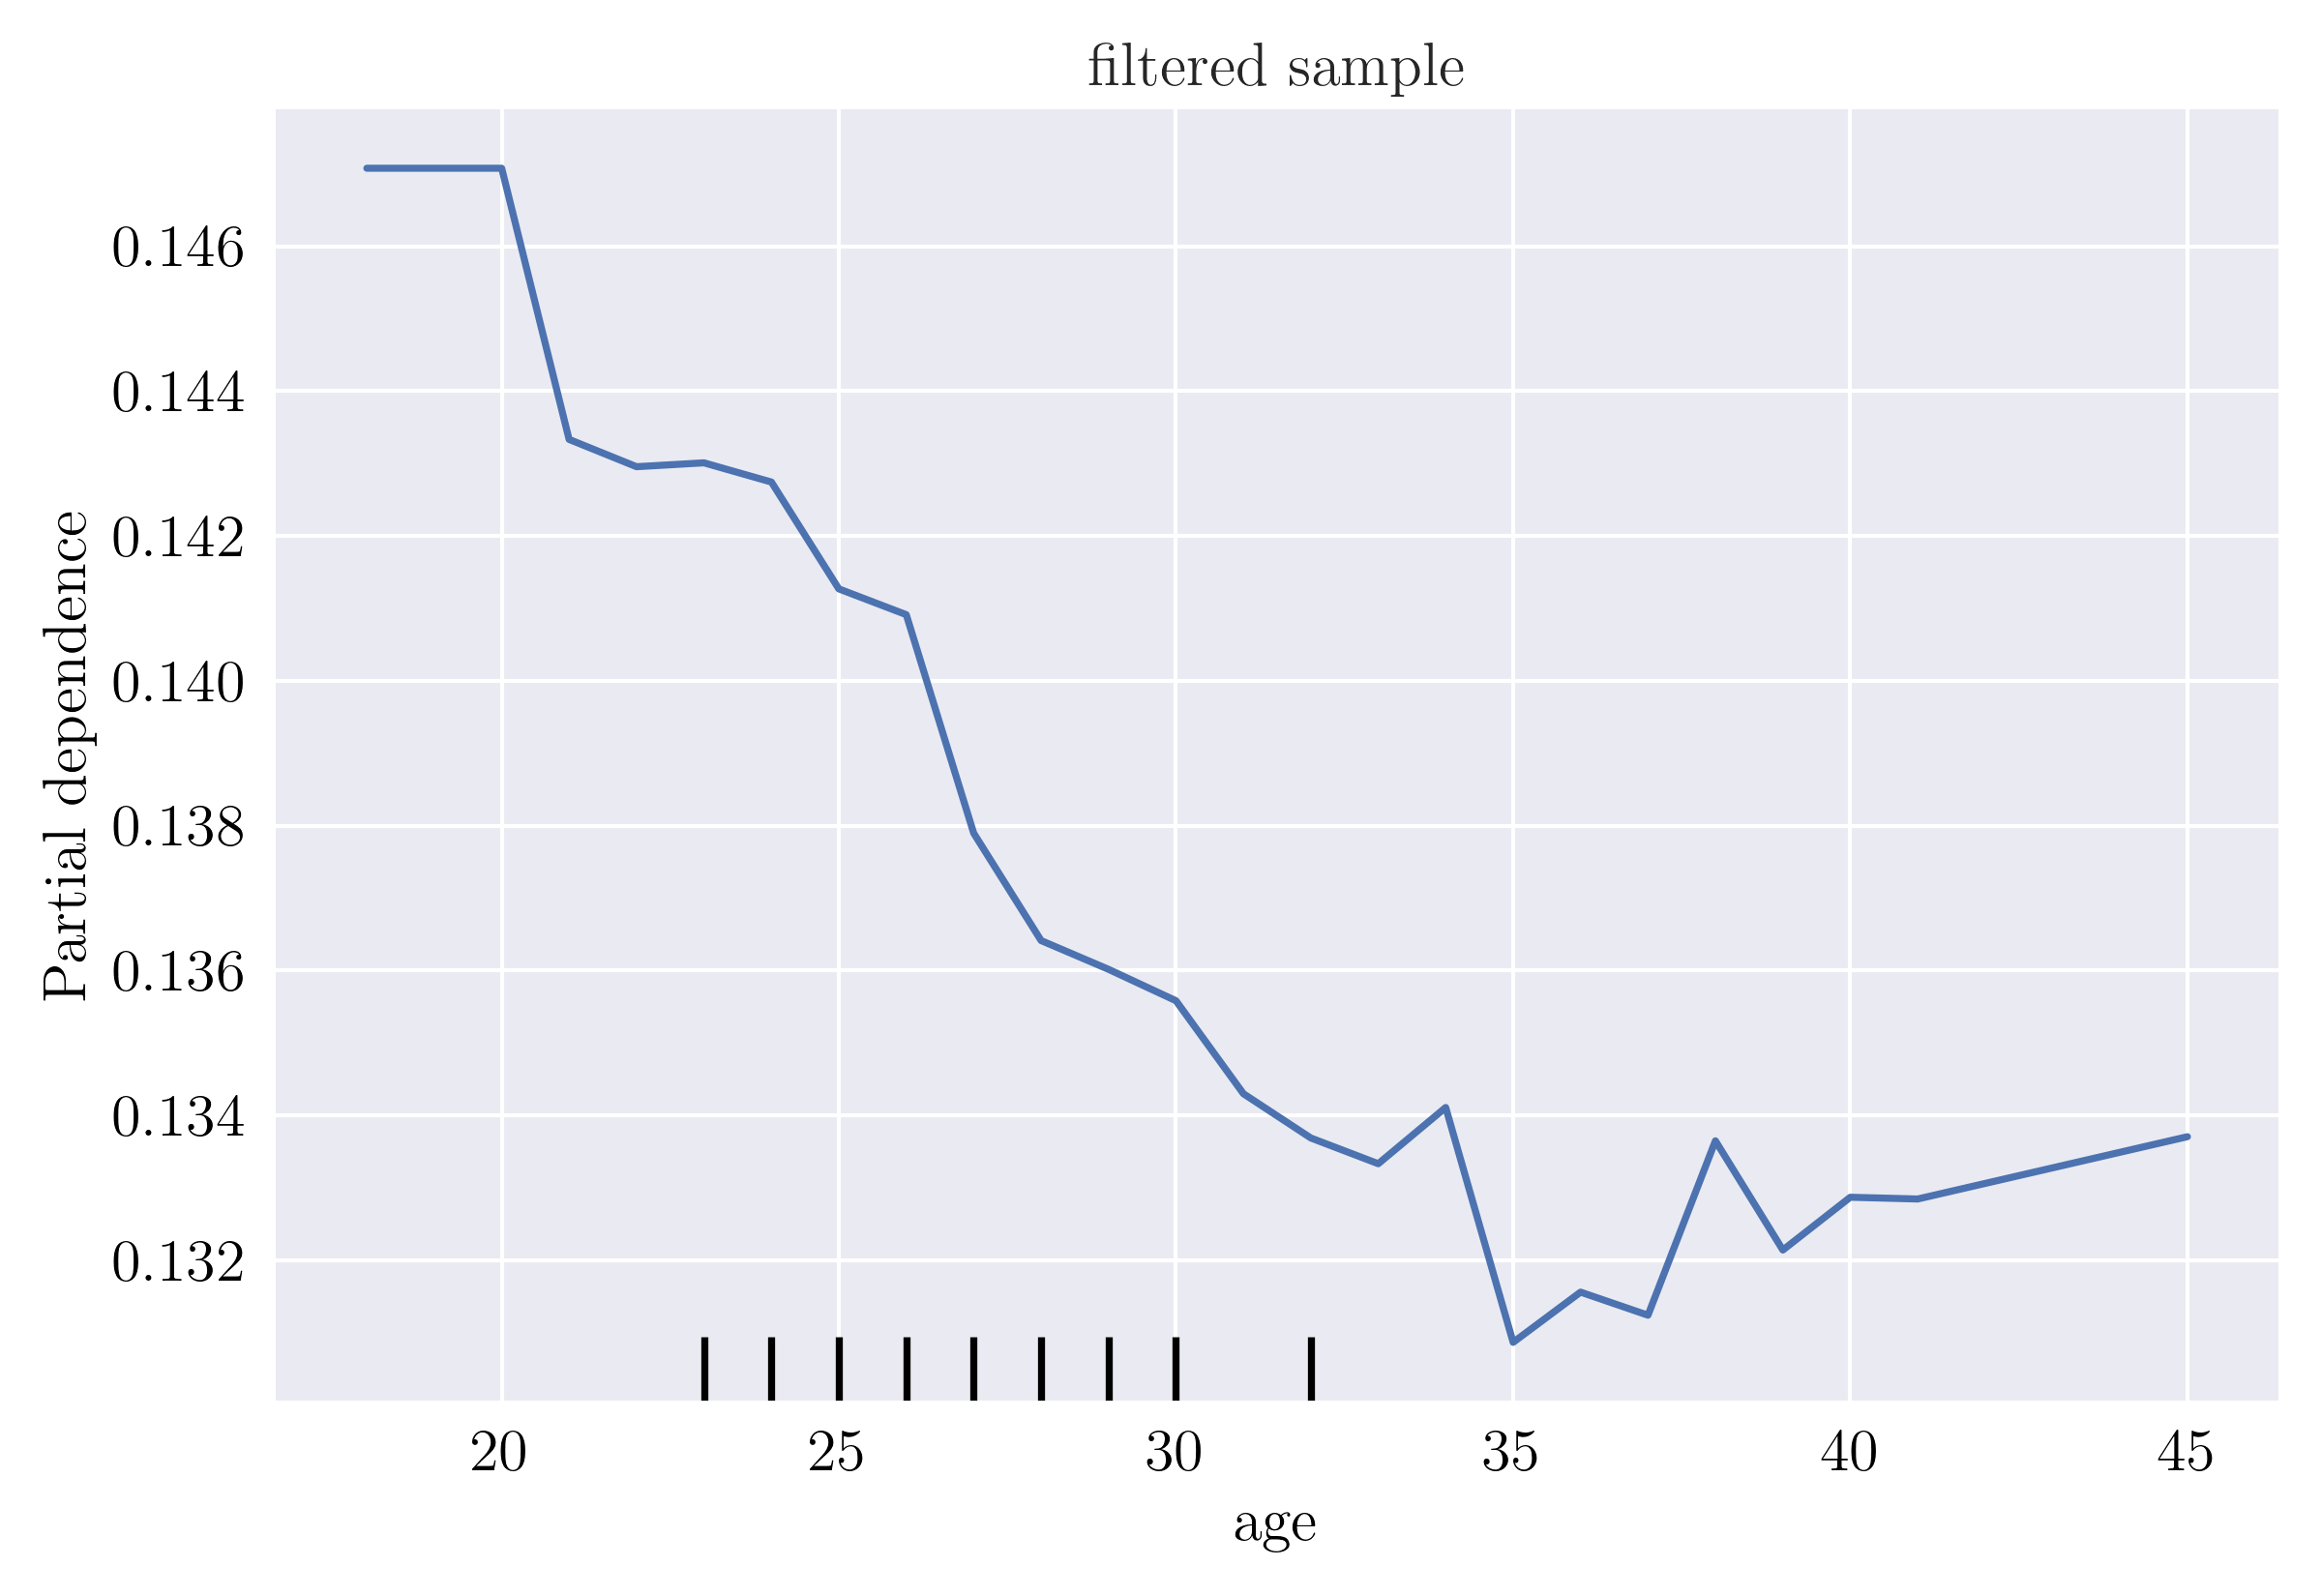
\includegraphics[width=0.49\linewidth]{attachments/machine-learning/pd_age_rf_filtered_sample.png}
    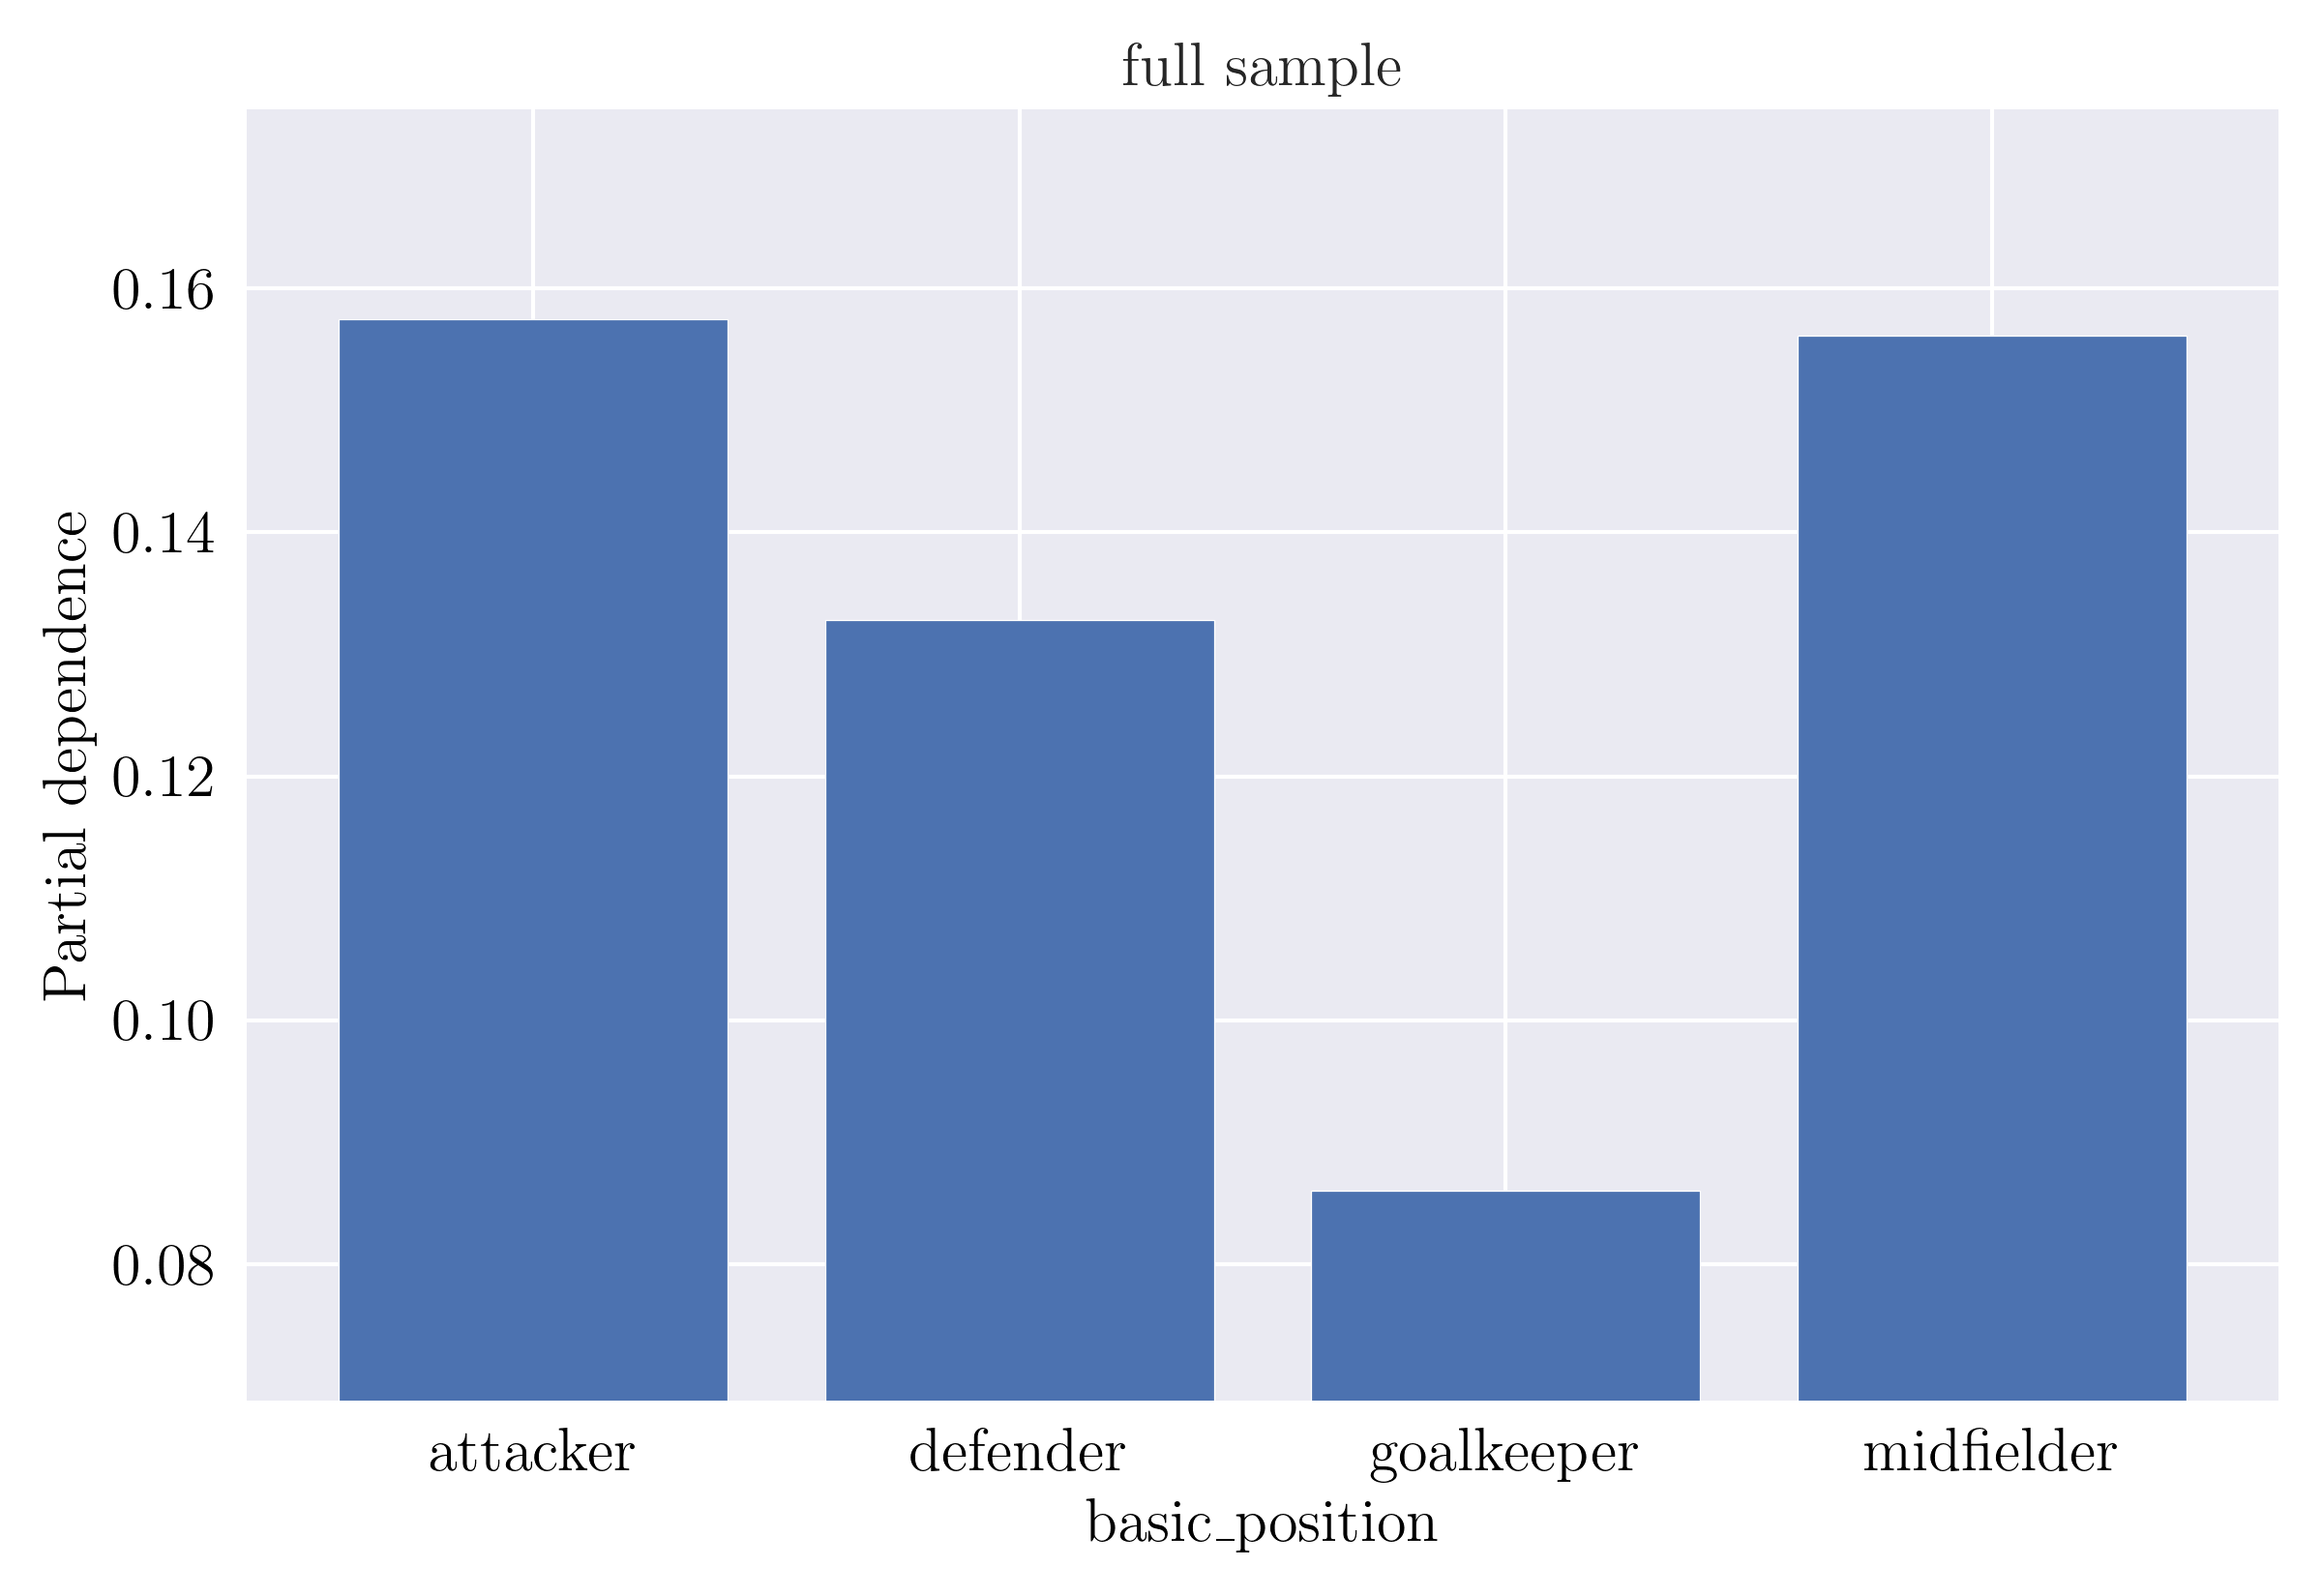
\includegraphics[width=0.49\linewidth]{attachments/machine-learning/pd_pos_rf_full_sample.png}
    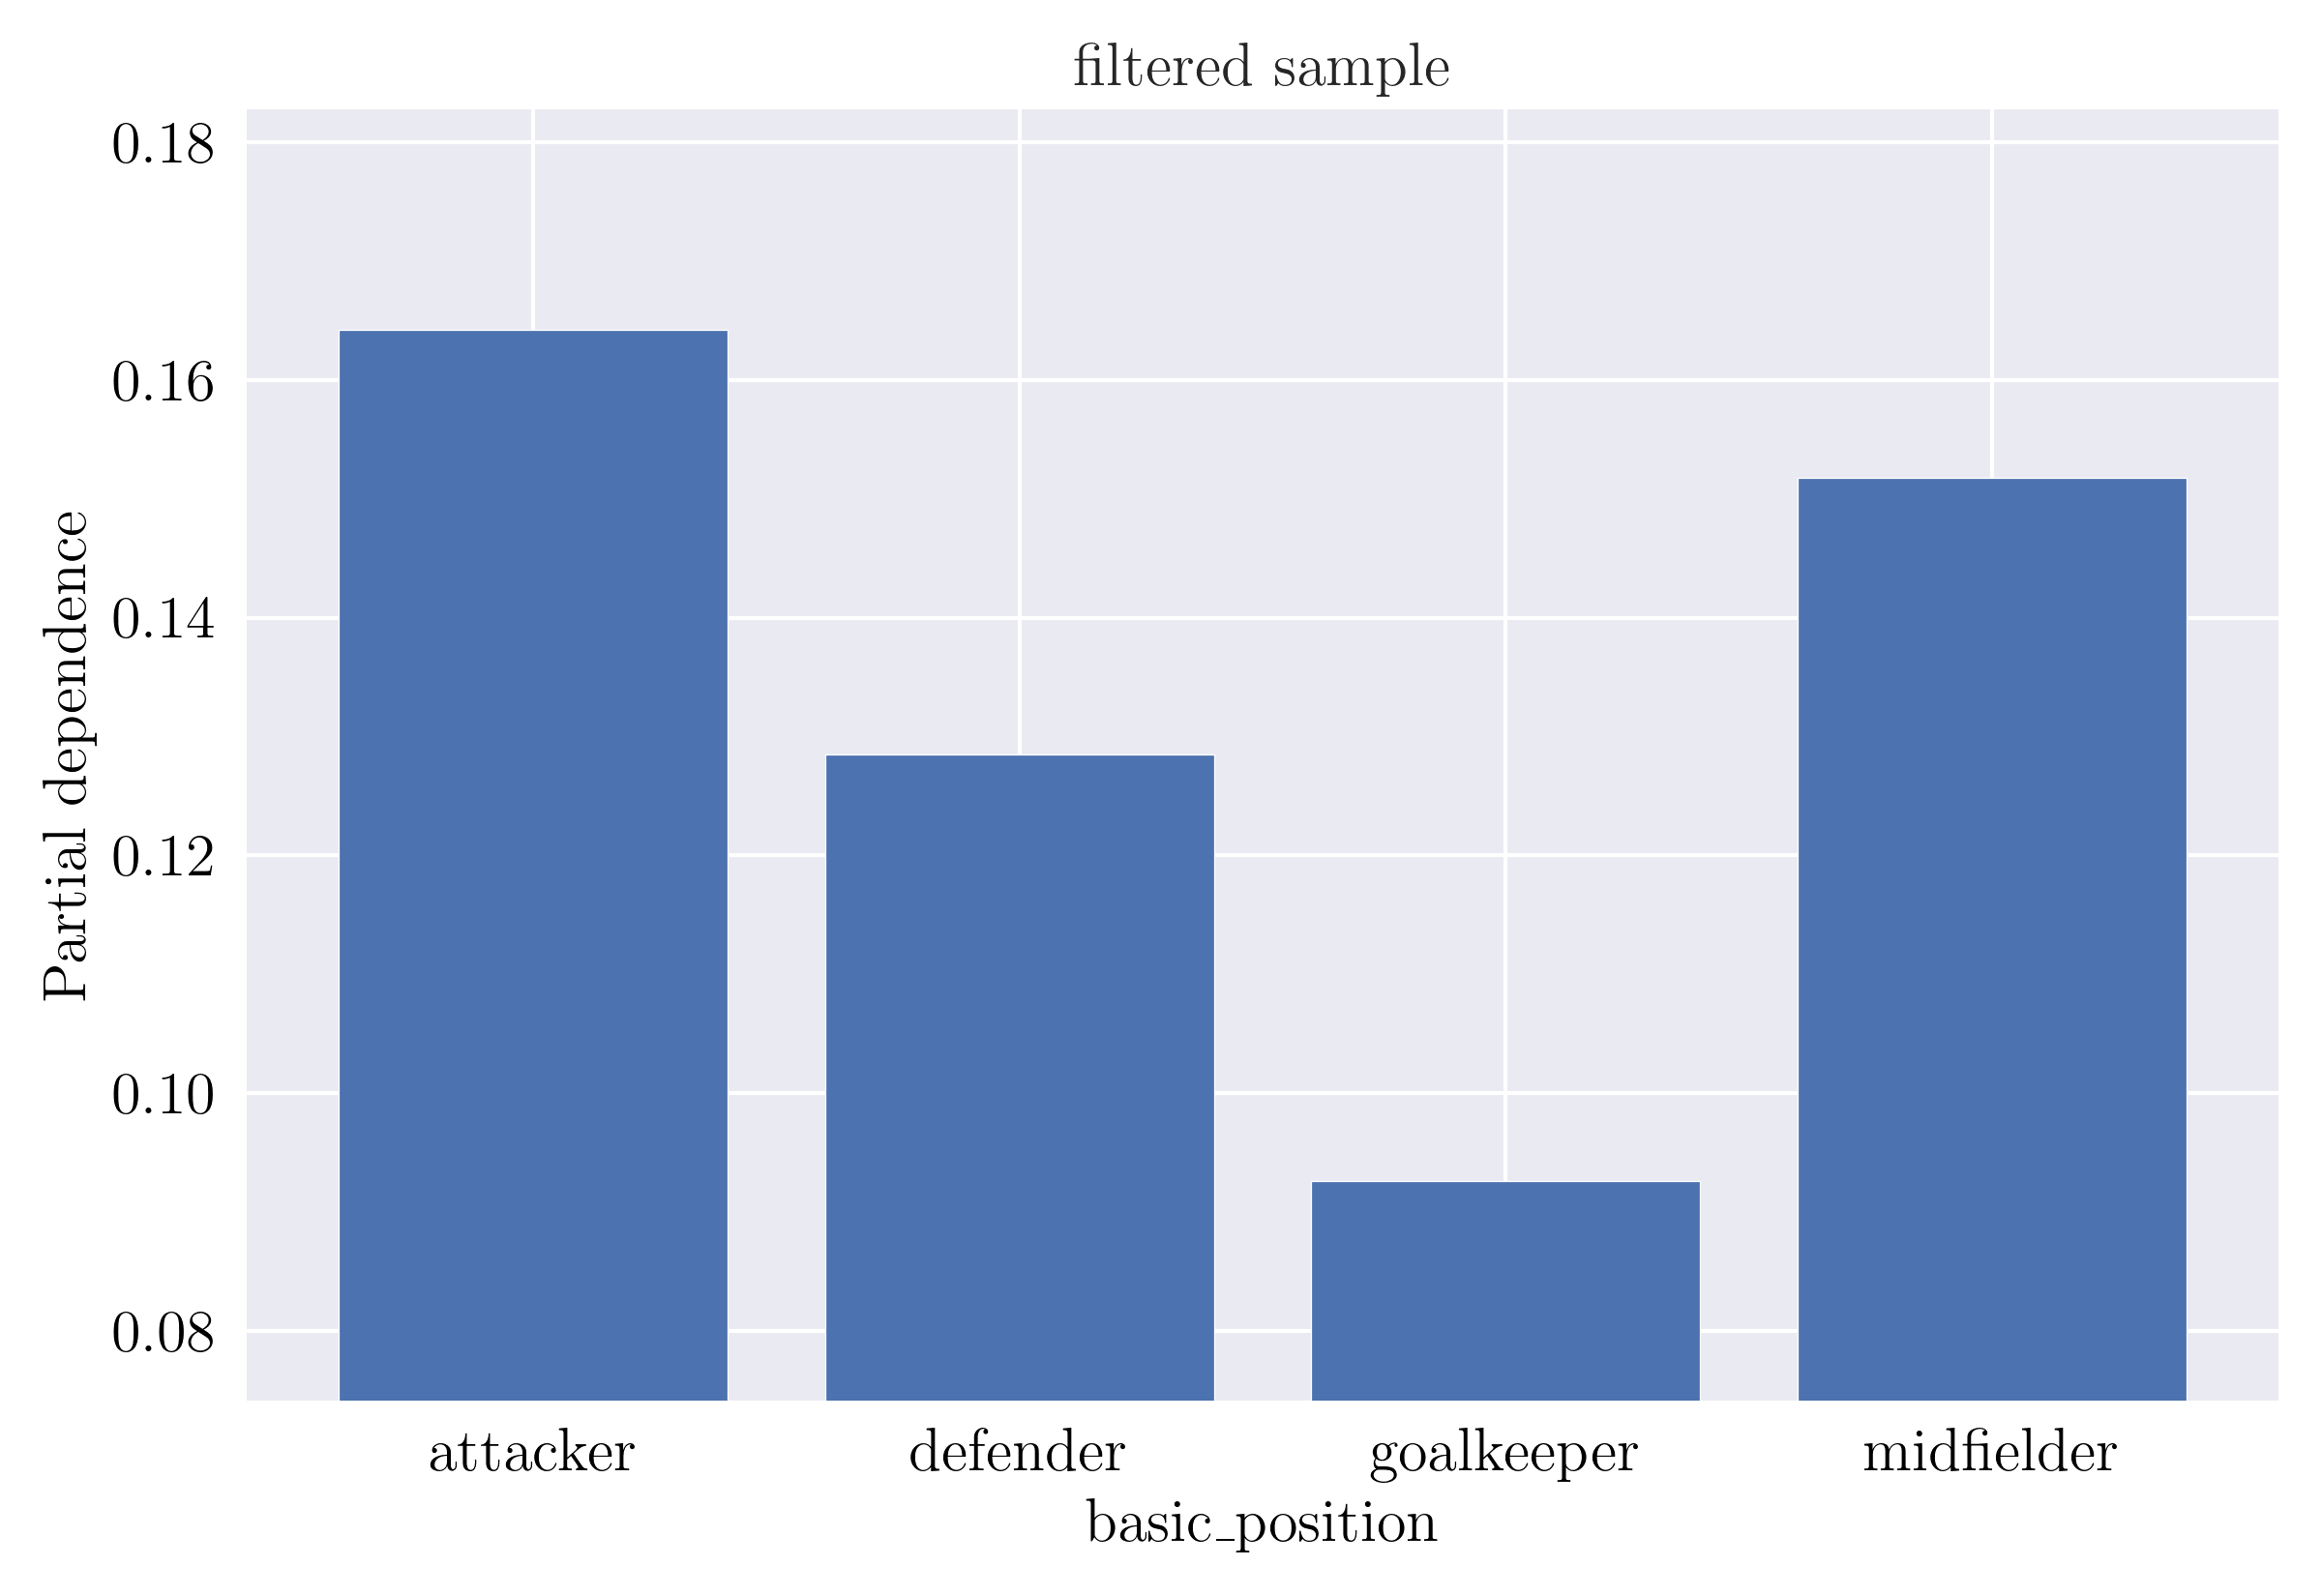
\includegraphics[width=0.49\linewidth]{attachments/machine-learning/pd_pos_rf_filtered_sample.png}
    \caption{Partial dependence plots for the effect of skill moves, age and playing position on the home advantage a player enjoys}
    \label{fig:pd_plots_2}
\end{figure}